\documentclass[a4paper, 11pt, titlepage]{jsarticle}
\usepackage[dvipdfmx]{graphicx}
\usepackage{amsmath}
\usepackage{listings}

\title{大学生リマインダー 仕様書}
\author{グループ3 カニと愉快な仲間たち\\215710B 深村芽紅\\215724B 高里優菜\\215726J 神村琉恩\\215746C 新垣樹}
\date{\today }

\begin{document}
\maketitle
\clearpage

\tableofcontents
\clearpage

\section{はじめに}
\subsection{目的}
本アプリケーションは、大学生の課題管理の効率化を目的として開発を行う。
\subsection{背景}
現在ネット上で公開されているリマインダーアプリは、個人・業務向けのものが多く、学生向けのリマインダーアプリが少ない。数少ない学生向けリマインダーアプリも有料機能の制限があり、大学生活で活用するのは難しいという問題がある。
\subsection{期待される効果}
学生向けのリマインダーを開発し、学生が利用することで、課題管理、スケジュール管理の効率化を図る。それにより、学生の計画性を高め、学習時間の増加や課外活動に取り組む時間の確保につなげる。

\section{要件定義}
\subsection{概要}
本アプリケーションには大きく5つの機能を実装する。
\begin{itemize}
\item 講義ごとの課題の管理機能
\item 課題の提出日を視覚化するカレンダー機能
\item 現在の出席状況を確認する出席確認機能
\item テスト、課題の点数から見込み評価を算出する機能
\item 課題締め切りの通知機能
\end{itemize}

\subsection{利用者}
大学生(学部生1年次〜4年次)を想定。

\clearpage

\subsection{機能要件}
機能要件は以下の通りとする。
\begin{table}[htbp]
  \centering
  {\scriptsize
  \begin{tabular}{|l|l|l|l|l|}
    \hline
    要件NO & 分類1 & 分類2 & 要件内容 & 重要度 \\ \hline \hline
    1 & 共通 & 利用者 & 利用者は大学生(1年次〜4年次)とする & 高\\ \hline
    2 & 共通 & 権限 & 利用者は、履修している講義情報の登録・編集・削除の権限が与えられる & 高\\ \hline
    3 & 共通 & 権限 & 利用者は、講義ごとに出される課題の追加、編集、削除の権限が与えられる & 高\\ \hline
    4 & 共通 & 利用環境 & パソコン(MacOS)から操作可能であること & 高\\ \hline
    5 & 通知 & 通知機能 & 課題の締め切りが近くなったらPC上で通知を行う & 高 \\ \hline
    6 & 出席 & 出席記録 & 利用者は、講義時間内に出席の記録が可能 & 高\\ \hline
    7 & 出席 & 出席記録 & 出席は講義時間内でしか記録できないものとする & 高\\ \hline
    8 & 保守機能 & 講義情報管理 & 過去に登録した講義情報を閲覧できるようにする & 中 \\ \hline
    9 & 算出 & 見込み評価算出 & テスト・課題の点数から見込み評価を算出できること & 高 \\ \hline
  \end{tabular}
  }
  \caption{機能要件}
  \label{tb:kinou}
\end{table}

\subsection{非機能要件}
非機能要件は以下の通りとする。
\begin{table}[htbp]
  \centering
  {\scriptsize
  \begin{tabular}{|l|l|l|l|}
    \hline
    NO & 分類 & 要件内容 & 重要度 \\ \hline \hline
    1 & 性能・拡張性 & アプリ利用者はPC1台につき1ユーザーとする & 高\\ \hline
    2 & 運用・保守性 & アプリ稼働時間はユーザーがアプリ利用を終了するまでとする & 高\\ \hline
    3 & 開発 & 使用言語はPythonとしVSCodeを使用して開発を行う & 高\\ \hline
    4 & 開発 & GUI作成はkivyを使用して開発を行う & 高 \\ \hline
    5 & 開発 & データベースはSQLiteを使用する & 高 \\ \hline
    6 & 開発 & バージョン管理はGitを使用する & 高\\ \hline
    7 & 開発 & 本アプリの開発手法は、ウォーターフォール型を基本として行う & 高\\ \hline
  \end{tabular}
  }
  \caption{非機能要件}
  \label{tb:n-kinou}
\end{table}

\subsection{情報・データ}
データ構成は以下の通りとする
\begin{itemize}
\item 講義情報
\begin{itemize}
  \item 講義名
  \item 講義時間
  \item 単位数
  \item 教室場所 or Zoom接続先リンク
  \item 教授情報
  \begin{itemize}
    \item 教授名
    \item 教授連絡先
  \end{itemize}
  \item 評価基準
  \begin{itemize}
    \item 課題評価比率
    \item 中間テスト評価比率
    \item 期末テスト評価比率
  \end{itemize}
\end{itemize}
\item 課題情報
\begin{itemize}
  \item 課題名
  \item 重要度
  \item 締切日
  \item 取組み予定日
\end{itemize}
\item 出席
\begin{itemize}
\item 出席数
\item 遅刻数
\item 欠席数
\end{itemize}
\end{itemize}


\subsection{スケジュール}
スケジュールは以下の通りとする。
\begin{itemize}
\item 7/15 要件定義、基本設計
\item 7/22 詳細設計、画面レイアウト作成、講義登録機能作成、講義一覧機能作成
\item 7/29 出席記録機能作成、課題カレンダー作成、通知機能作成
\item 8/4 app化、提出
\item 8/5 プレゼン
\end{itemize}

\subsection{役割分担}
役割分担は以下の通りとする。
\begin{itemize}
\item 215710B 深村芽紅 - UIデザイナー
\item 215724B 高里優菜 - UIデザイナー 兼 プログラマー
\item 215726J 神村琉恩 - プログラマー 兼 リーダー
\item 215746C 新垣樹 - UIデザイナー 兼 プログラマー
\end{itemize}

\clearpage

\section{基本設計}
\subsection{機能設計}
\subsubsection{履修講義情報管理機能}
利用者が履修している講義内容の登録・編集・閲覧・削除を行う。
講義ごとに「講義名」「講義時間」「単位数」「教室場所 or Zoom接続先リンク」「教授情報」「評価基準」の情報を登録する。
\subsubsection{課題管理機能}
利用者に課せられた課題を講義ごとに追加・編集・閲覧・削除を行う。課題ごとに「課題名」「重要度」「締切日」「取組み予定日」の情報を記録する。課題取組み後はチェックをつけると、課題一覧から非表示になる。
\subsubsection{課題視覚化機能}
登録されている課題の締切をカレンダー形式で表示し視覚化する。
カレンダーは週間、月間、年間の表示の切り替えが可能。
カレンダー上に表示されている課題を選択すると、課題の詳細な情報を表示する。
\subsubsection{出席管理機能}
講義ごとの出席の記録・閲覧を行う。
出席は講義時間内にしか記録できないものとし、講義開始15分以内の記録で「出席」として記録。講義開始30分以内の記録で「遅刻」、それ以降を「欠席」として記録する。
\subsubsection{課題締切通知機能}
課題締切が近づくとPC上に通知を行う機能。
通知は1週間前、3日前、前日、当日の6時間前に行う。
\subsubsection{見込み評定算出機能}
課題・テストの点数を記録し、講義ごとの評価基準に基づき、見込み評価を算出する機能。評価基準は履修講義情報に記録されている情報を使用する。

\clearpage

\subsection{画面仕様}
\subsubsection{トップページ(出席記録ページ)}
\begin{figure}[htbp]
\begin{center}
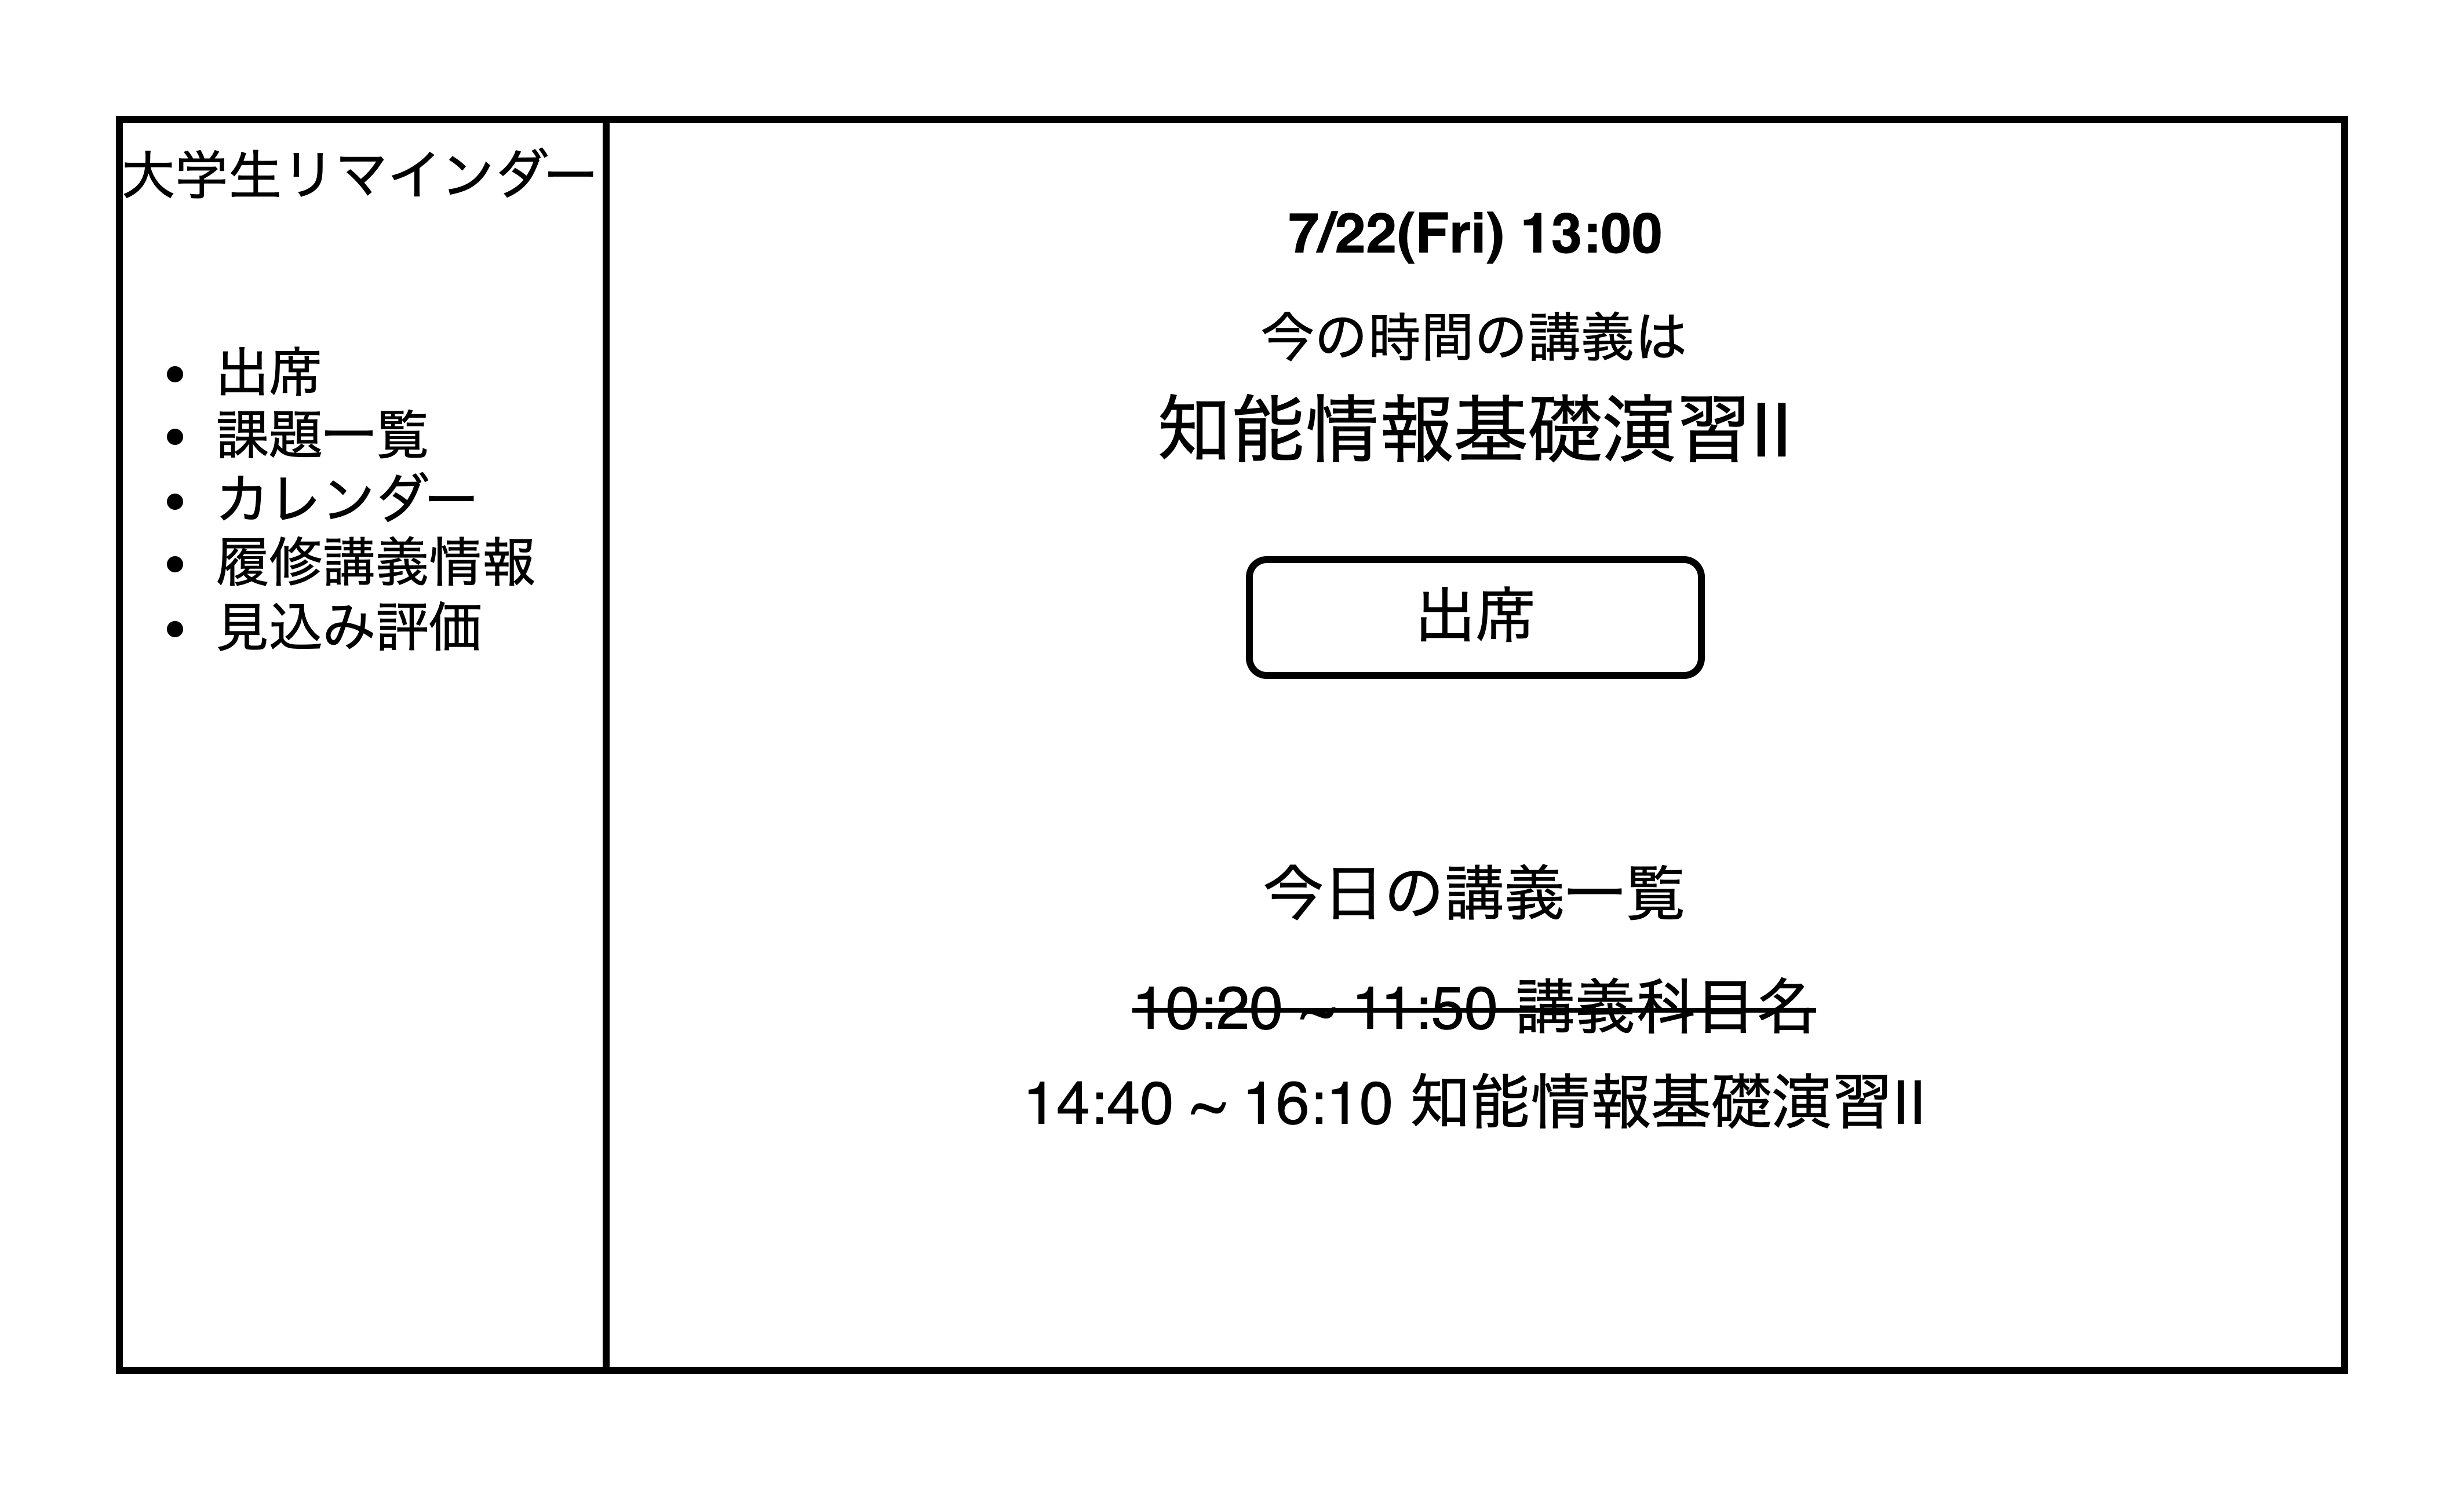
\includegraphics[width=120mm]{./img/Top.png}
\caption{トップページ(出席記録ページ)}
\end{center}
\end{figure}

\clearpage

\subsubsection{課題管理ページ}
\begin{figure}[htbp]
\begin{center}
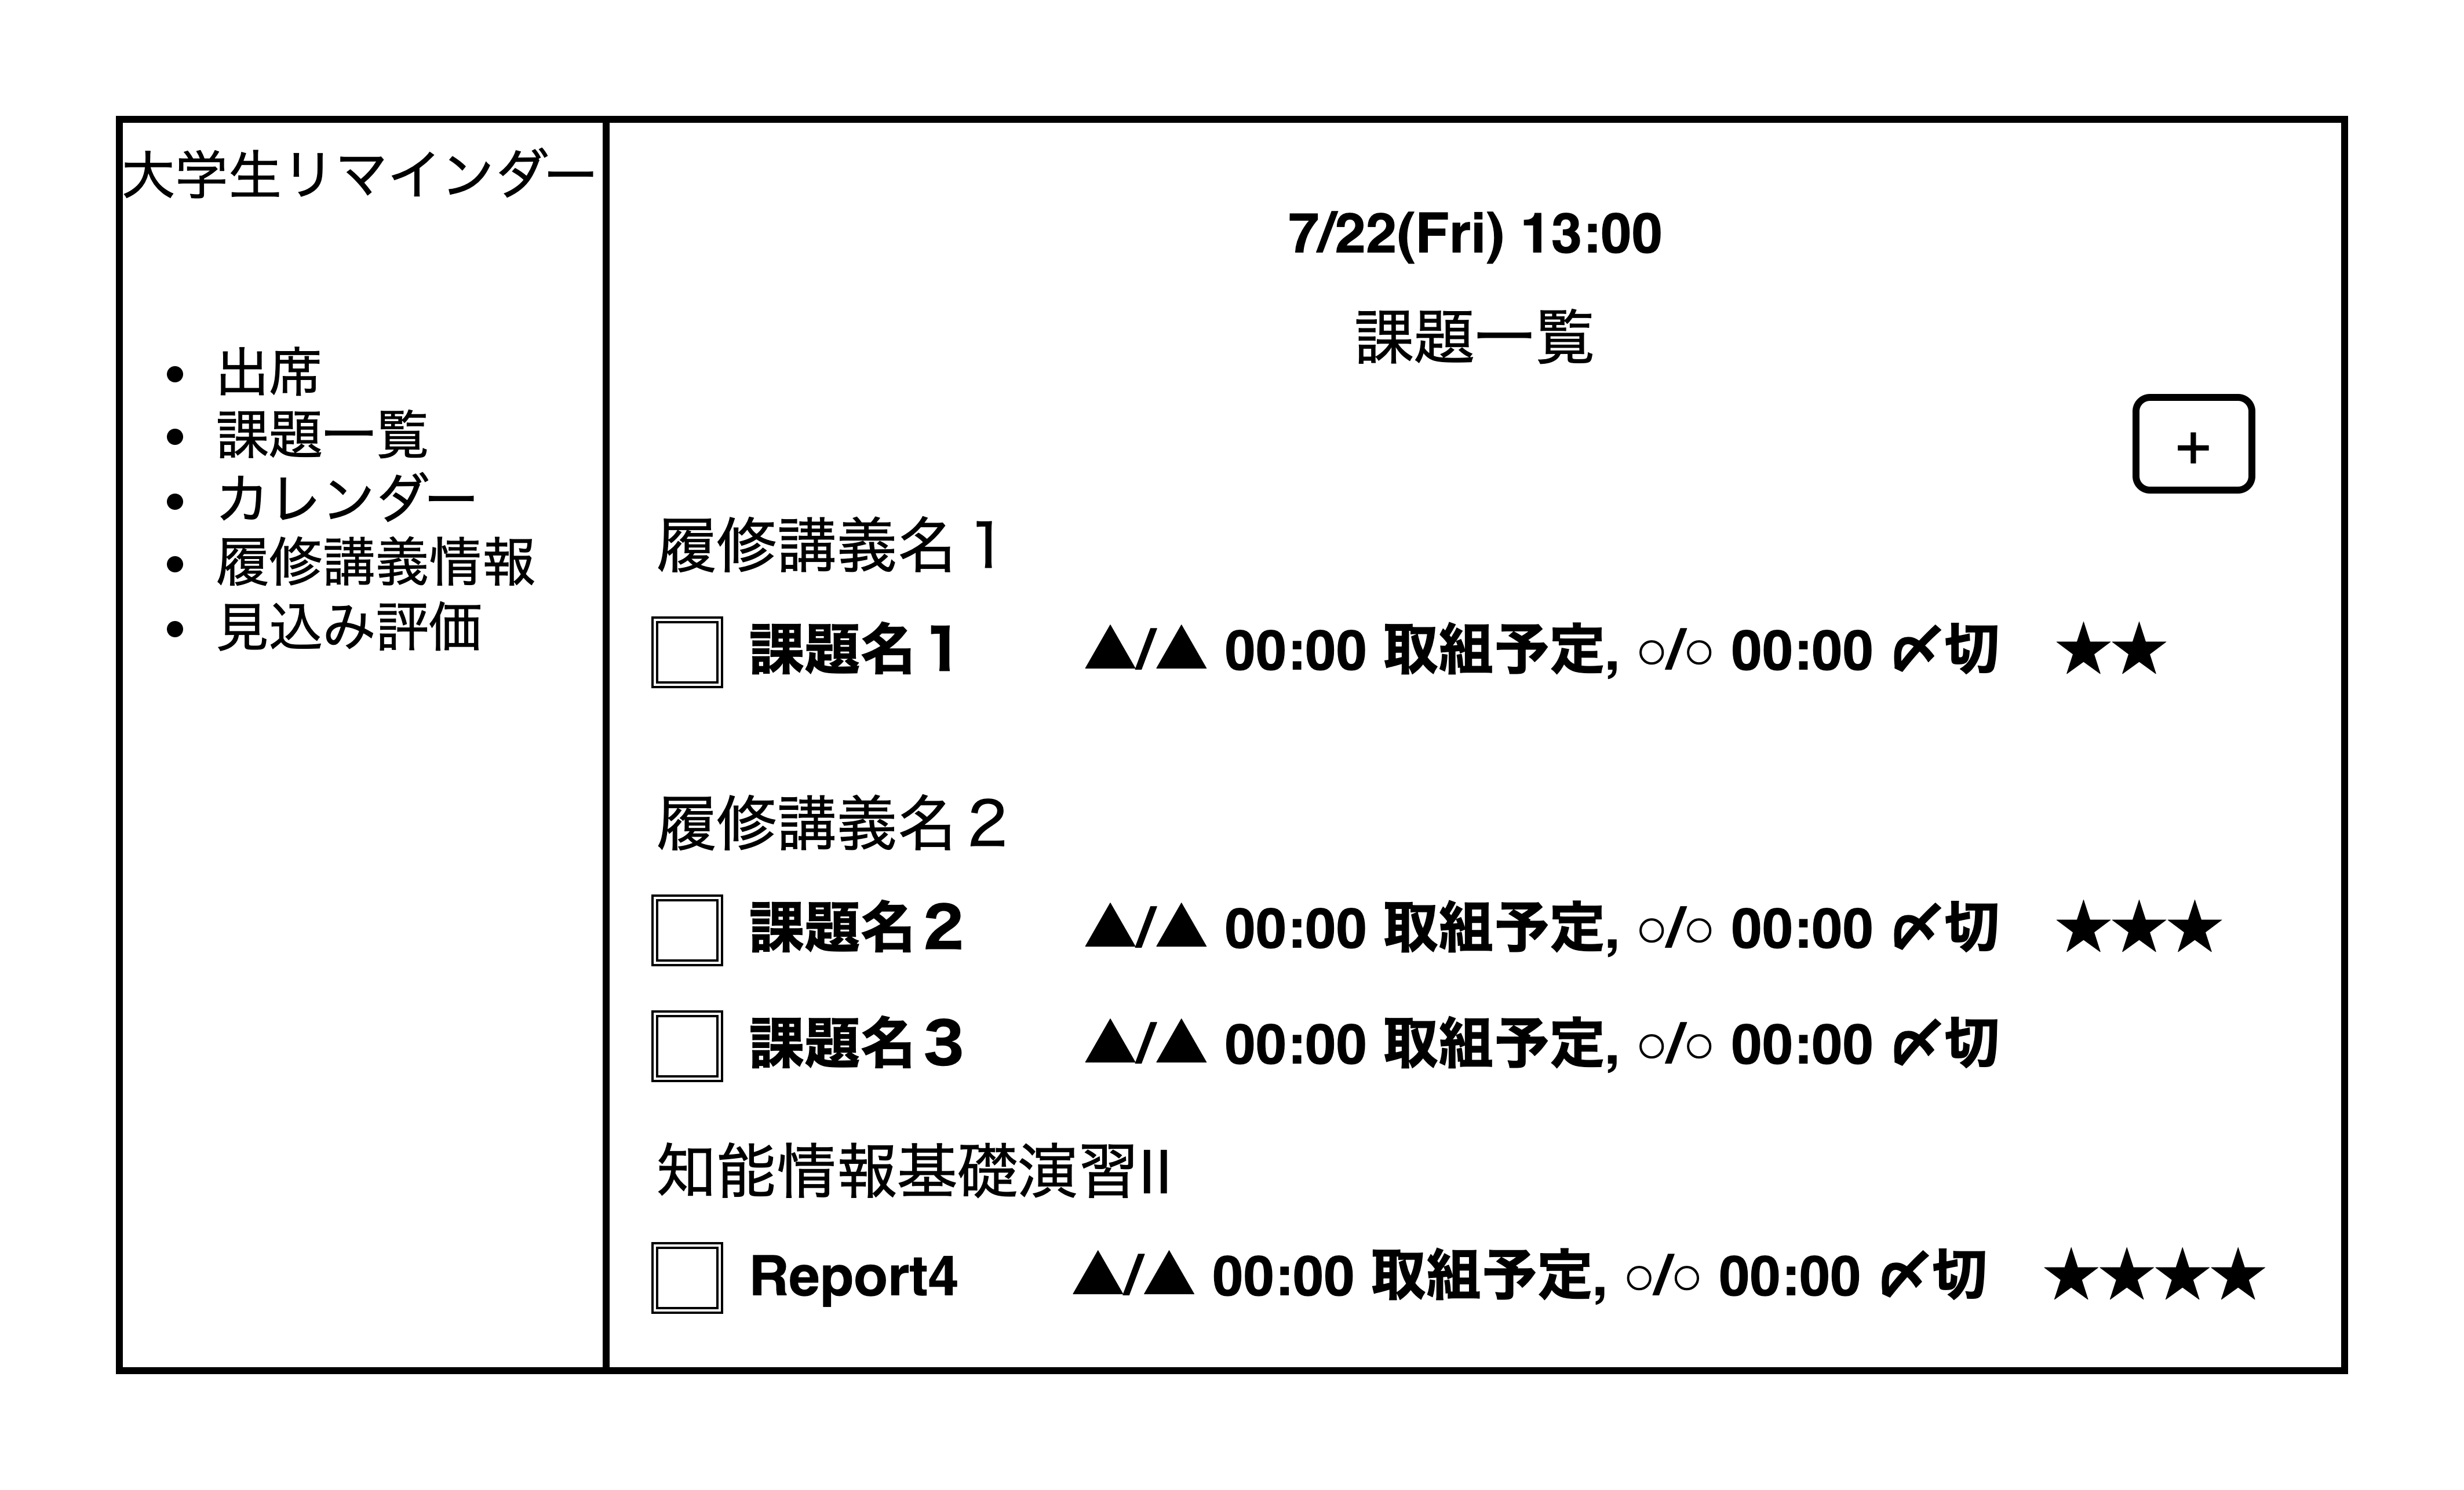
\includegraphics[width=120mm]{./img/Task1.png}
\caption{課題管理ページ(課題一覧)}
\end{center}
\end{figure}
\begin{figure}[htbp]
\begin{center}
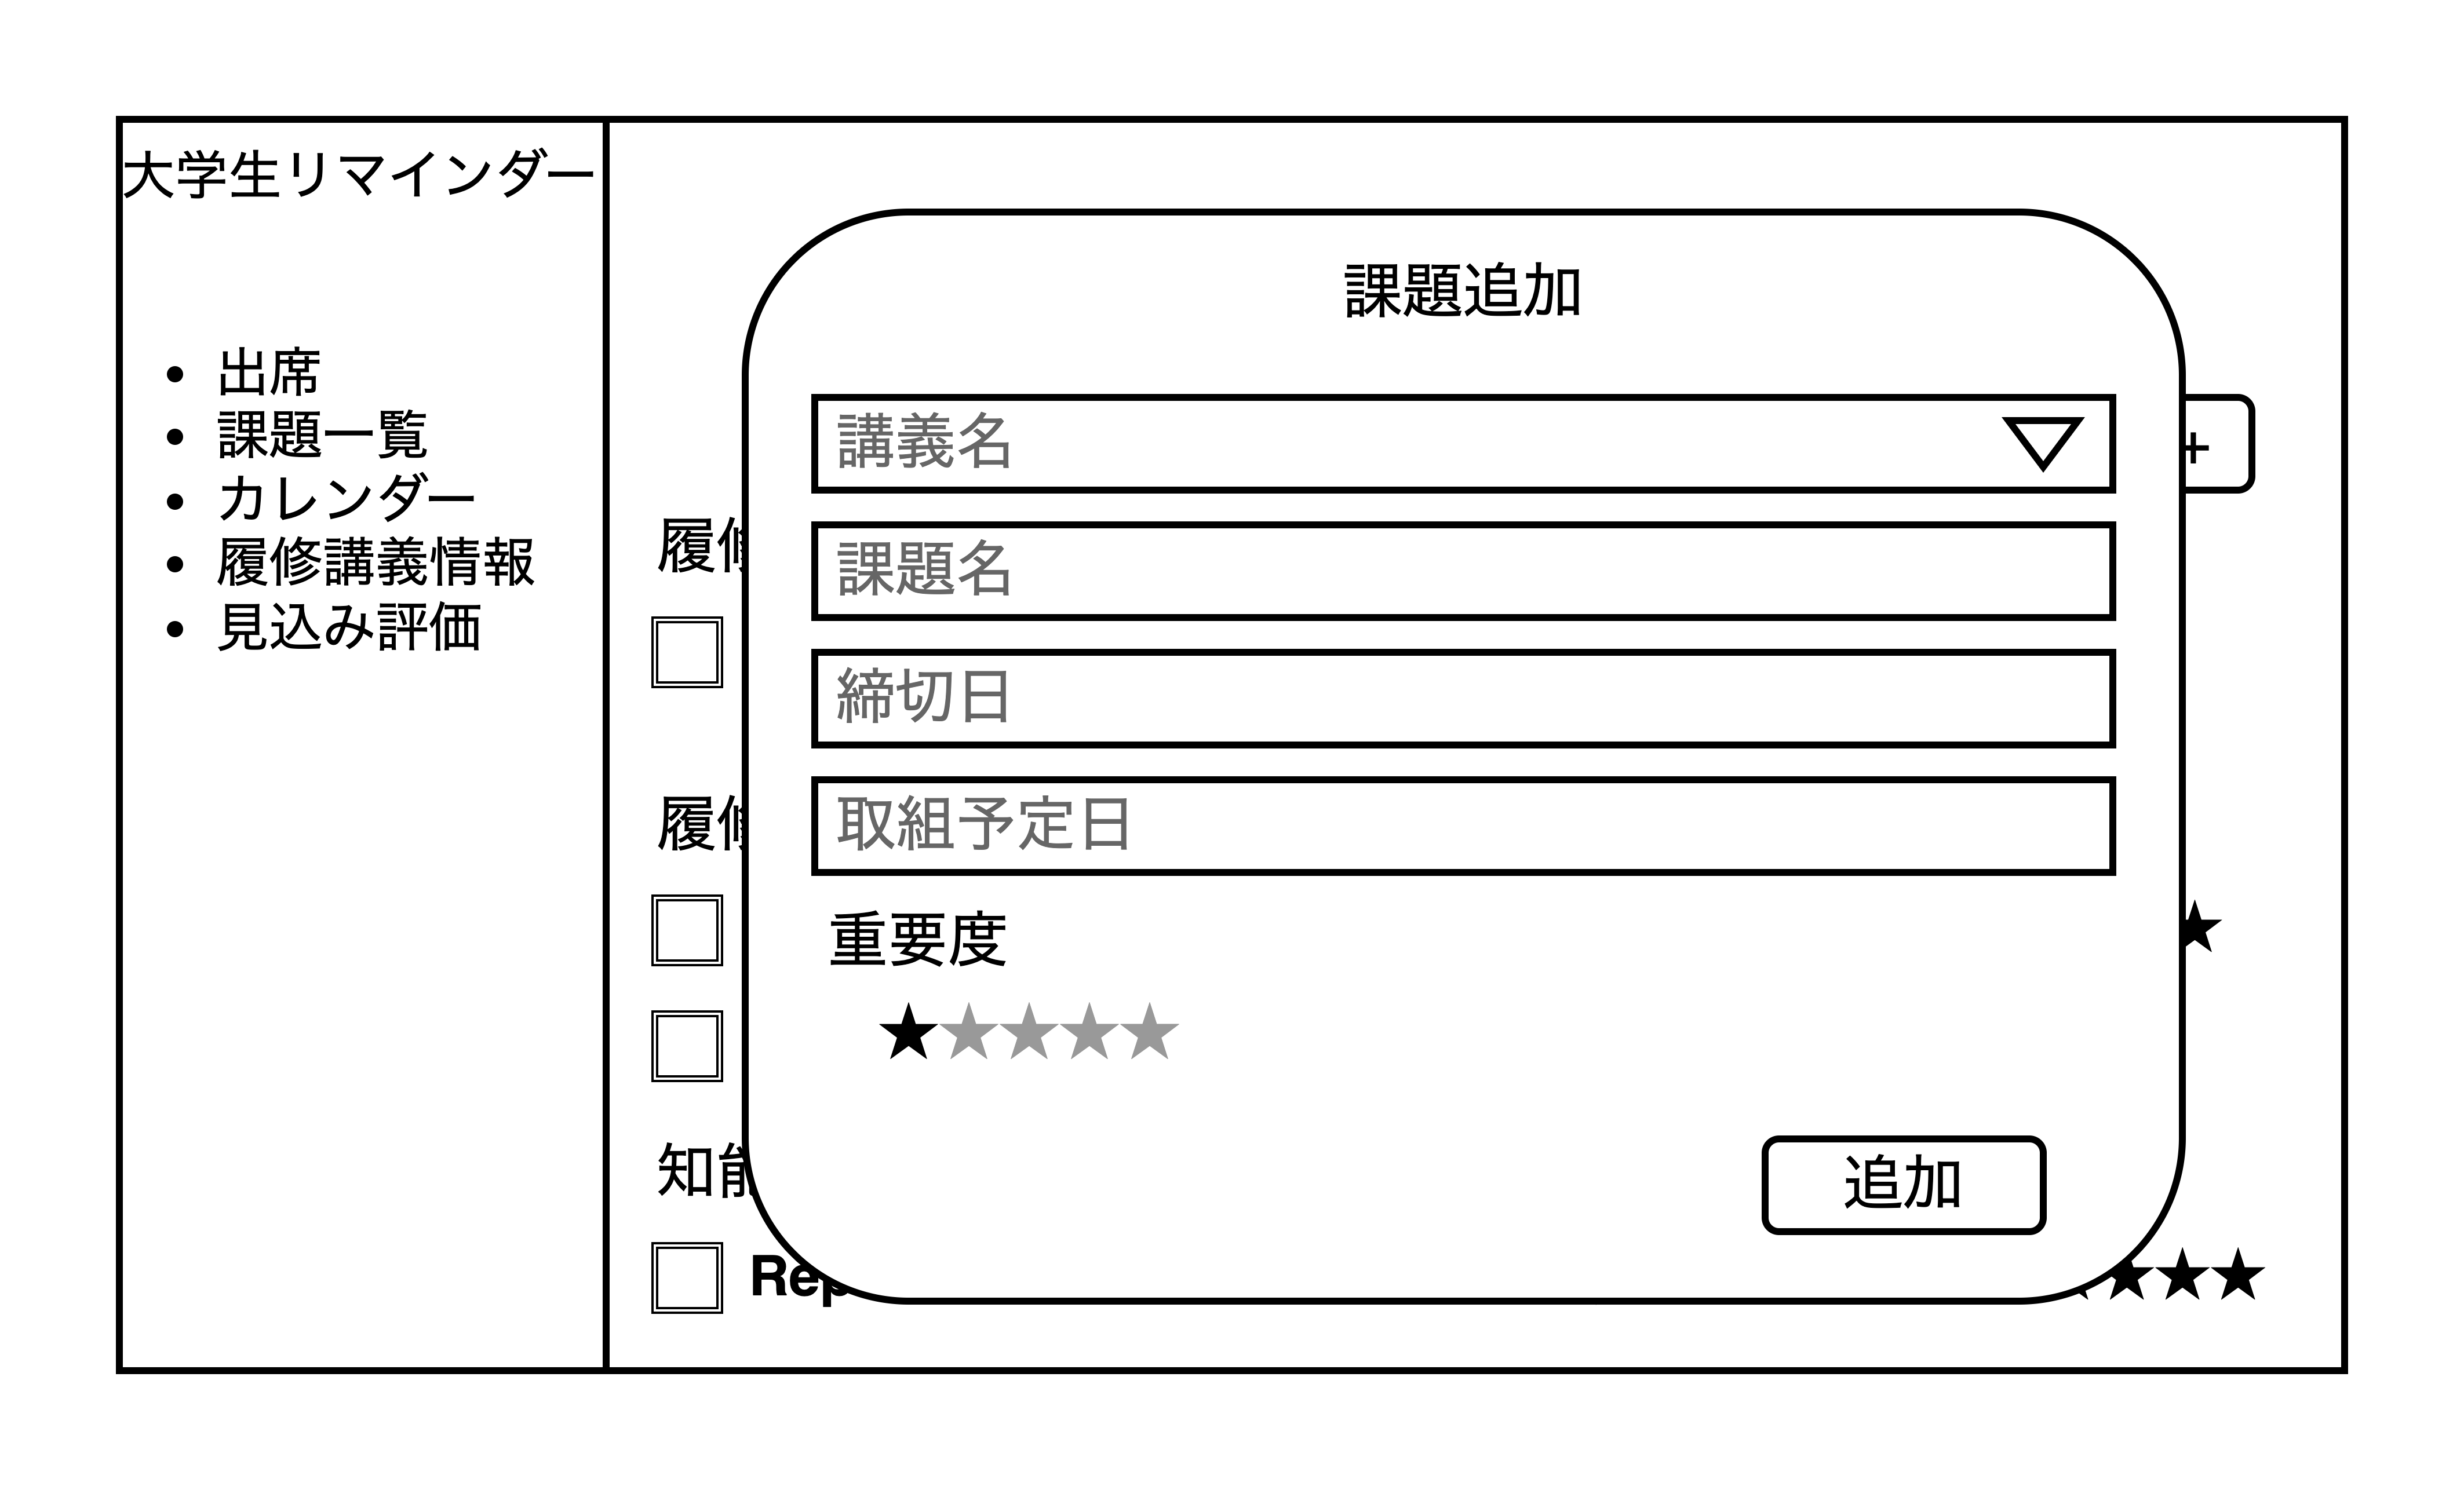
\includegraphics[width=120mm]{./img/Task2.png}
\caption{課題管理ページ(課題追加)}
\end{center}
\end{figure}

\clearpage

\subsubsection{カレンダーページ}
\begin{figure}[htbp]
\begin{center}
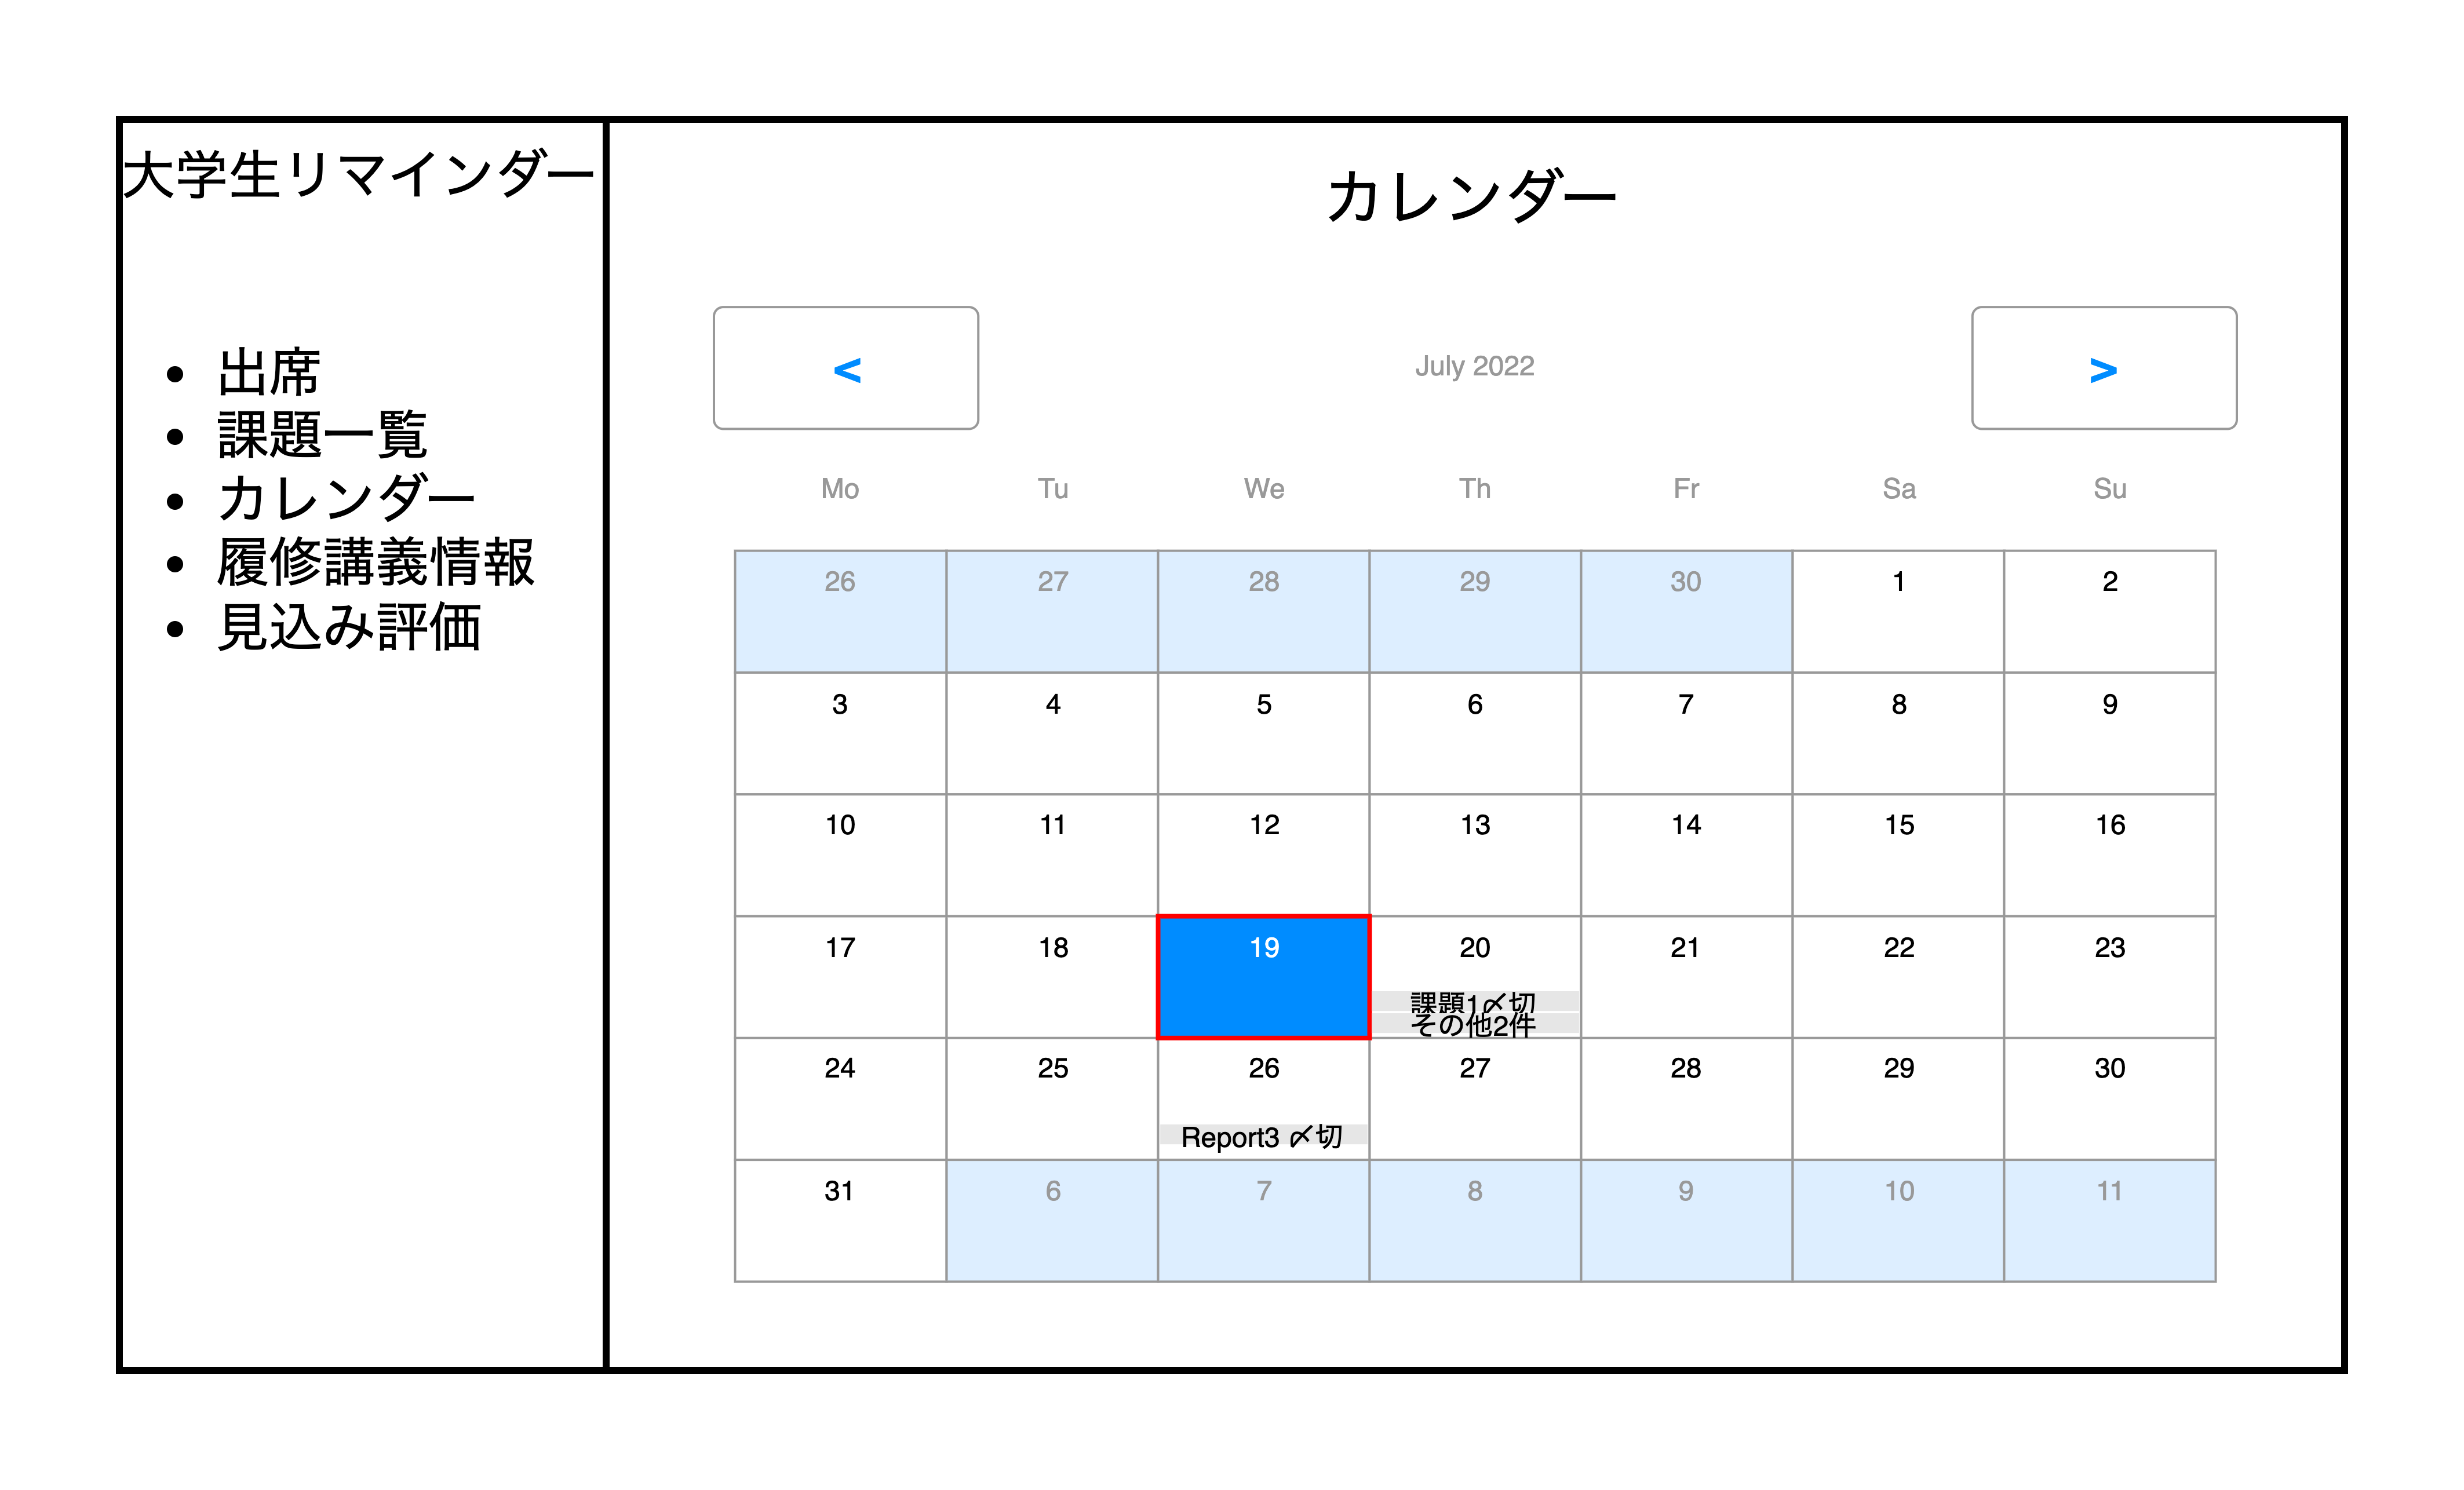
\includegraphics[width=120mm]{./img/Calendar1.png}
\caption{課題管理ページ(閲覧)}
\end{center}
\end{figure}
\begin{figure}[htbp]
\begin{center}
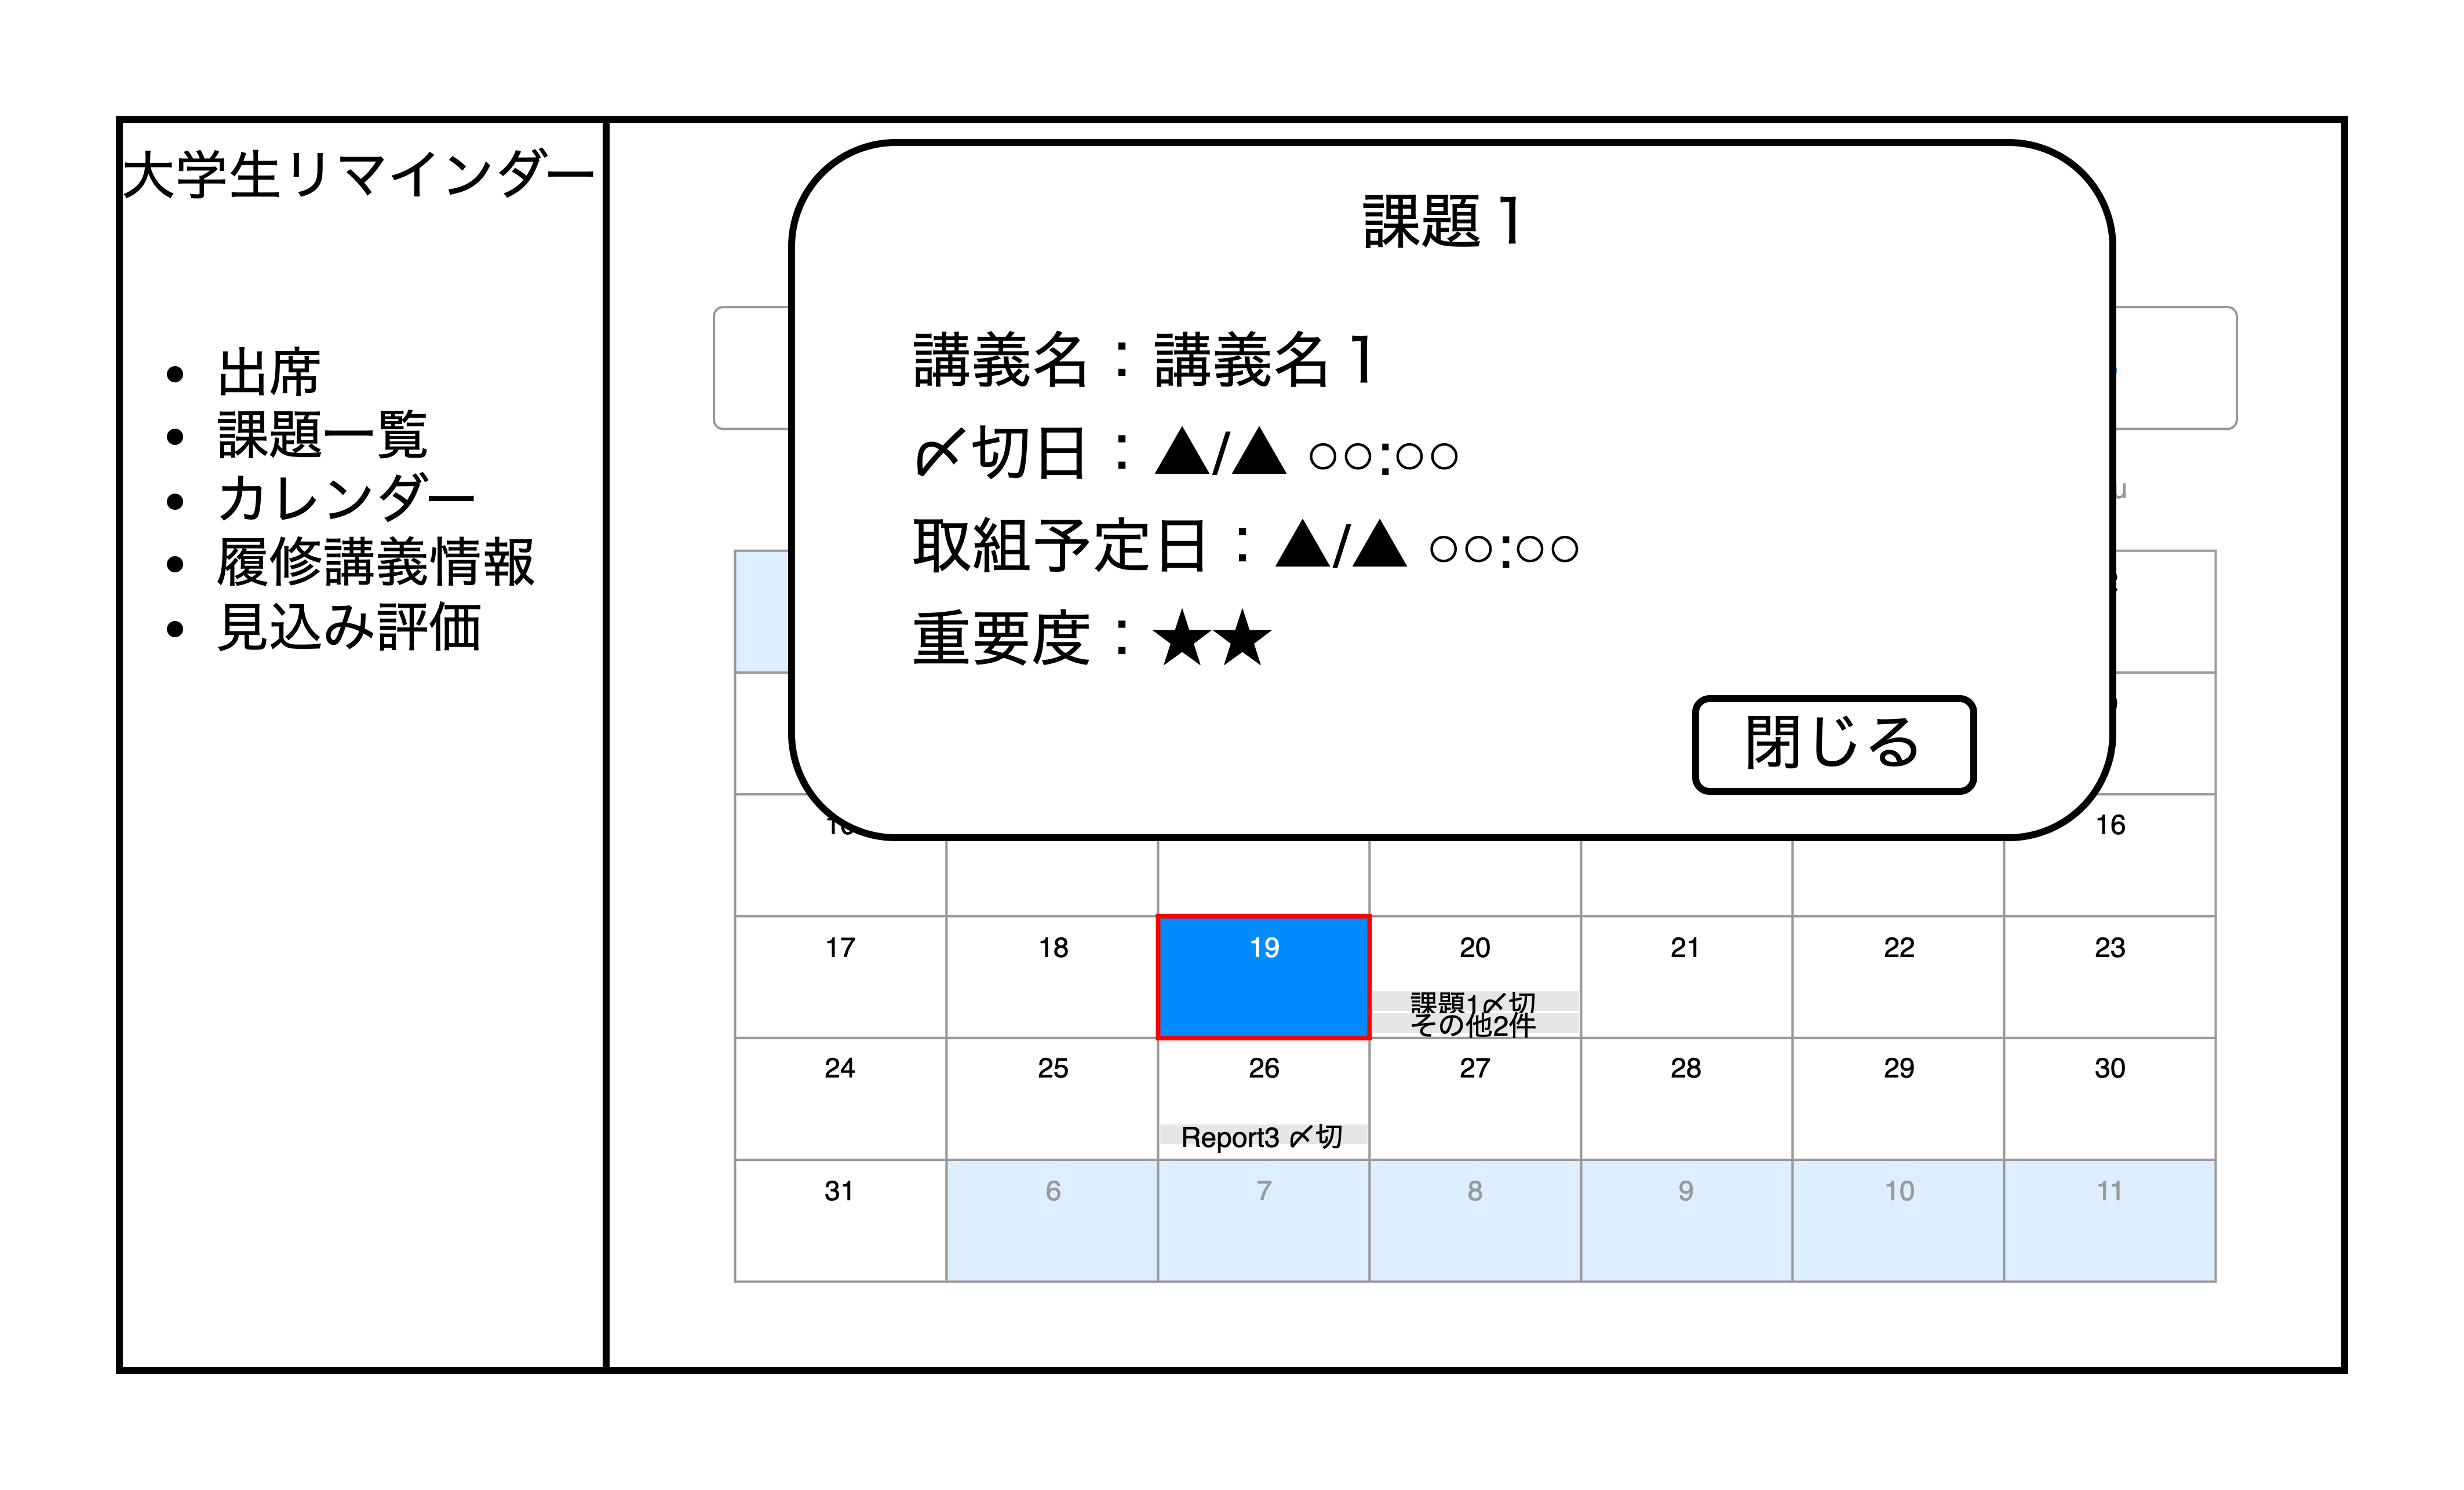
\includegraphics[width=120mm]{./img/Calendar2.png}
\caption{課題管理ページ(課題詳細)}
\end{center}
\end{figure}

\clearpage

\subsubsection{履修講義情報ページ}
\begin{figure}[htbp]
\begin{center}
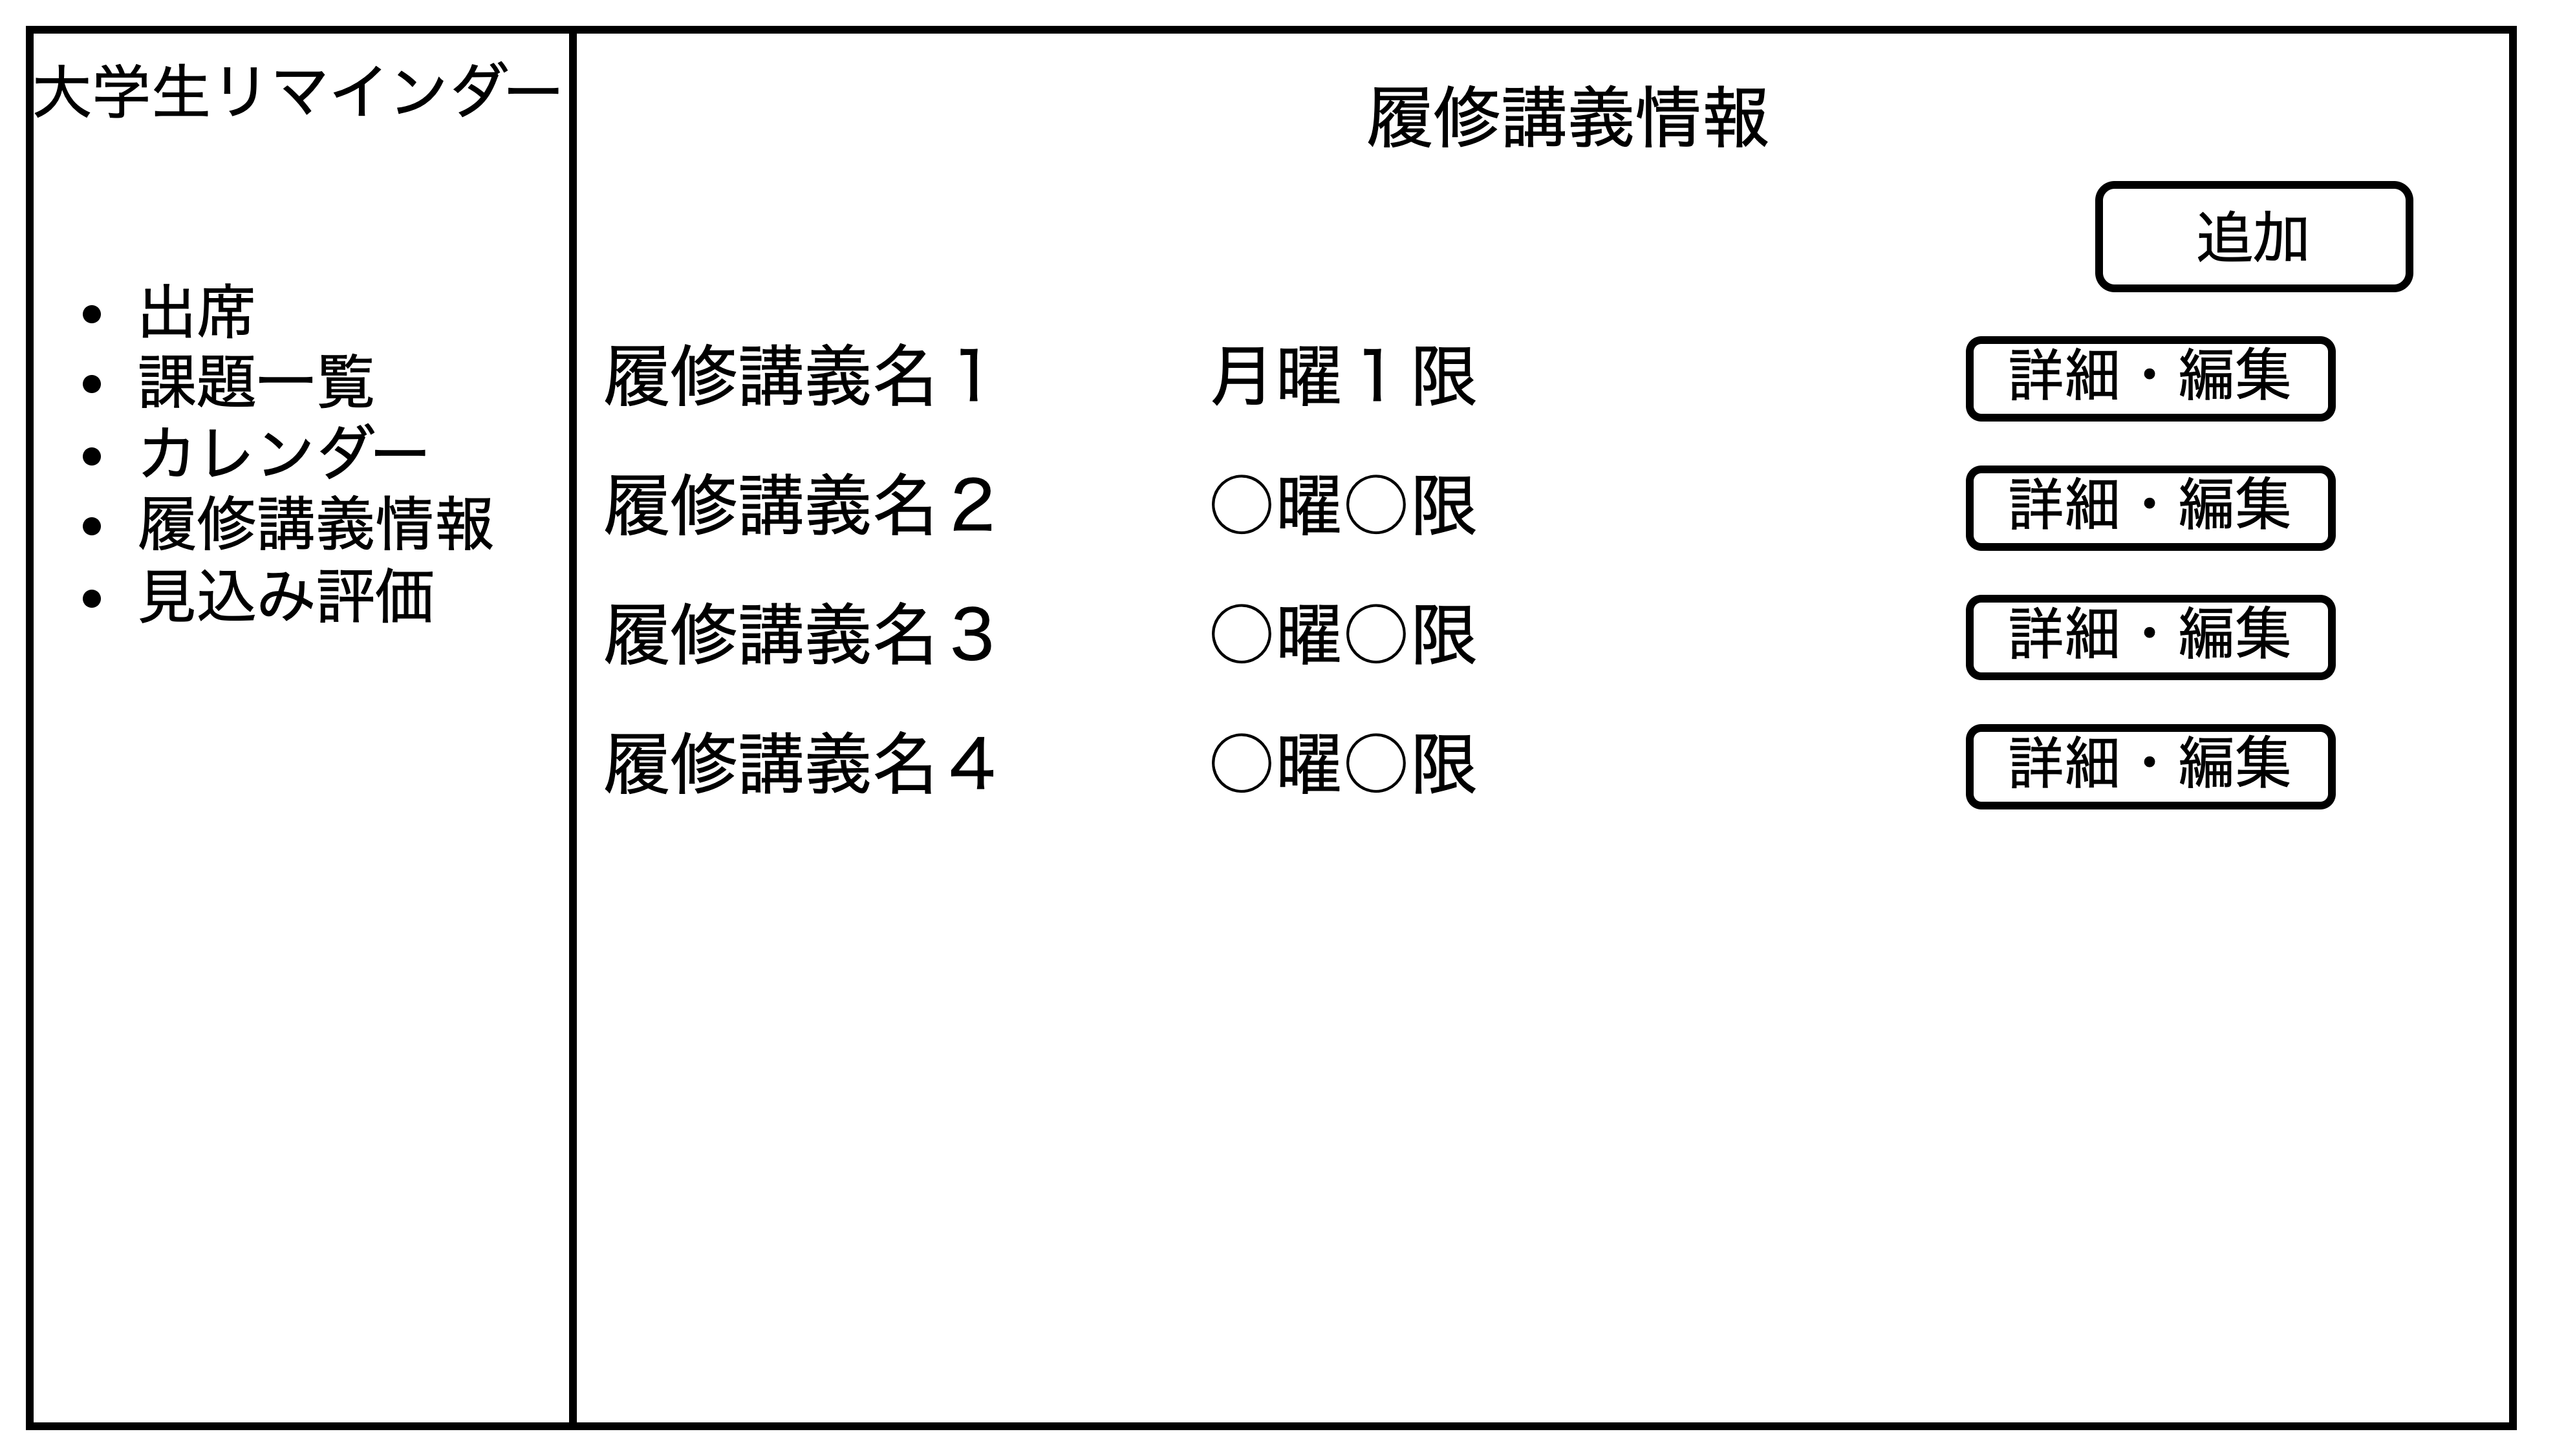
\includegraphics[width=120mm]{./img/Lecture1.png}
\caption{履修講義情報ページ(閲覧)}
\end{center}
\end{figure}
\begin{figure}[htbp]
\begin{center}
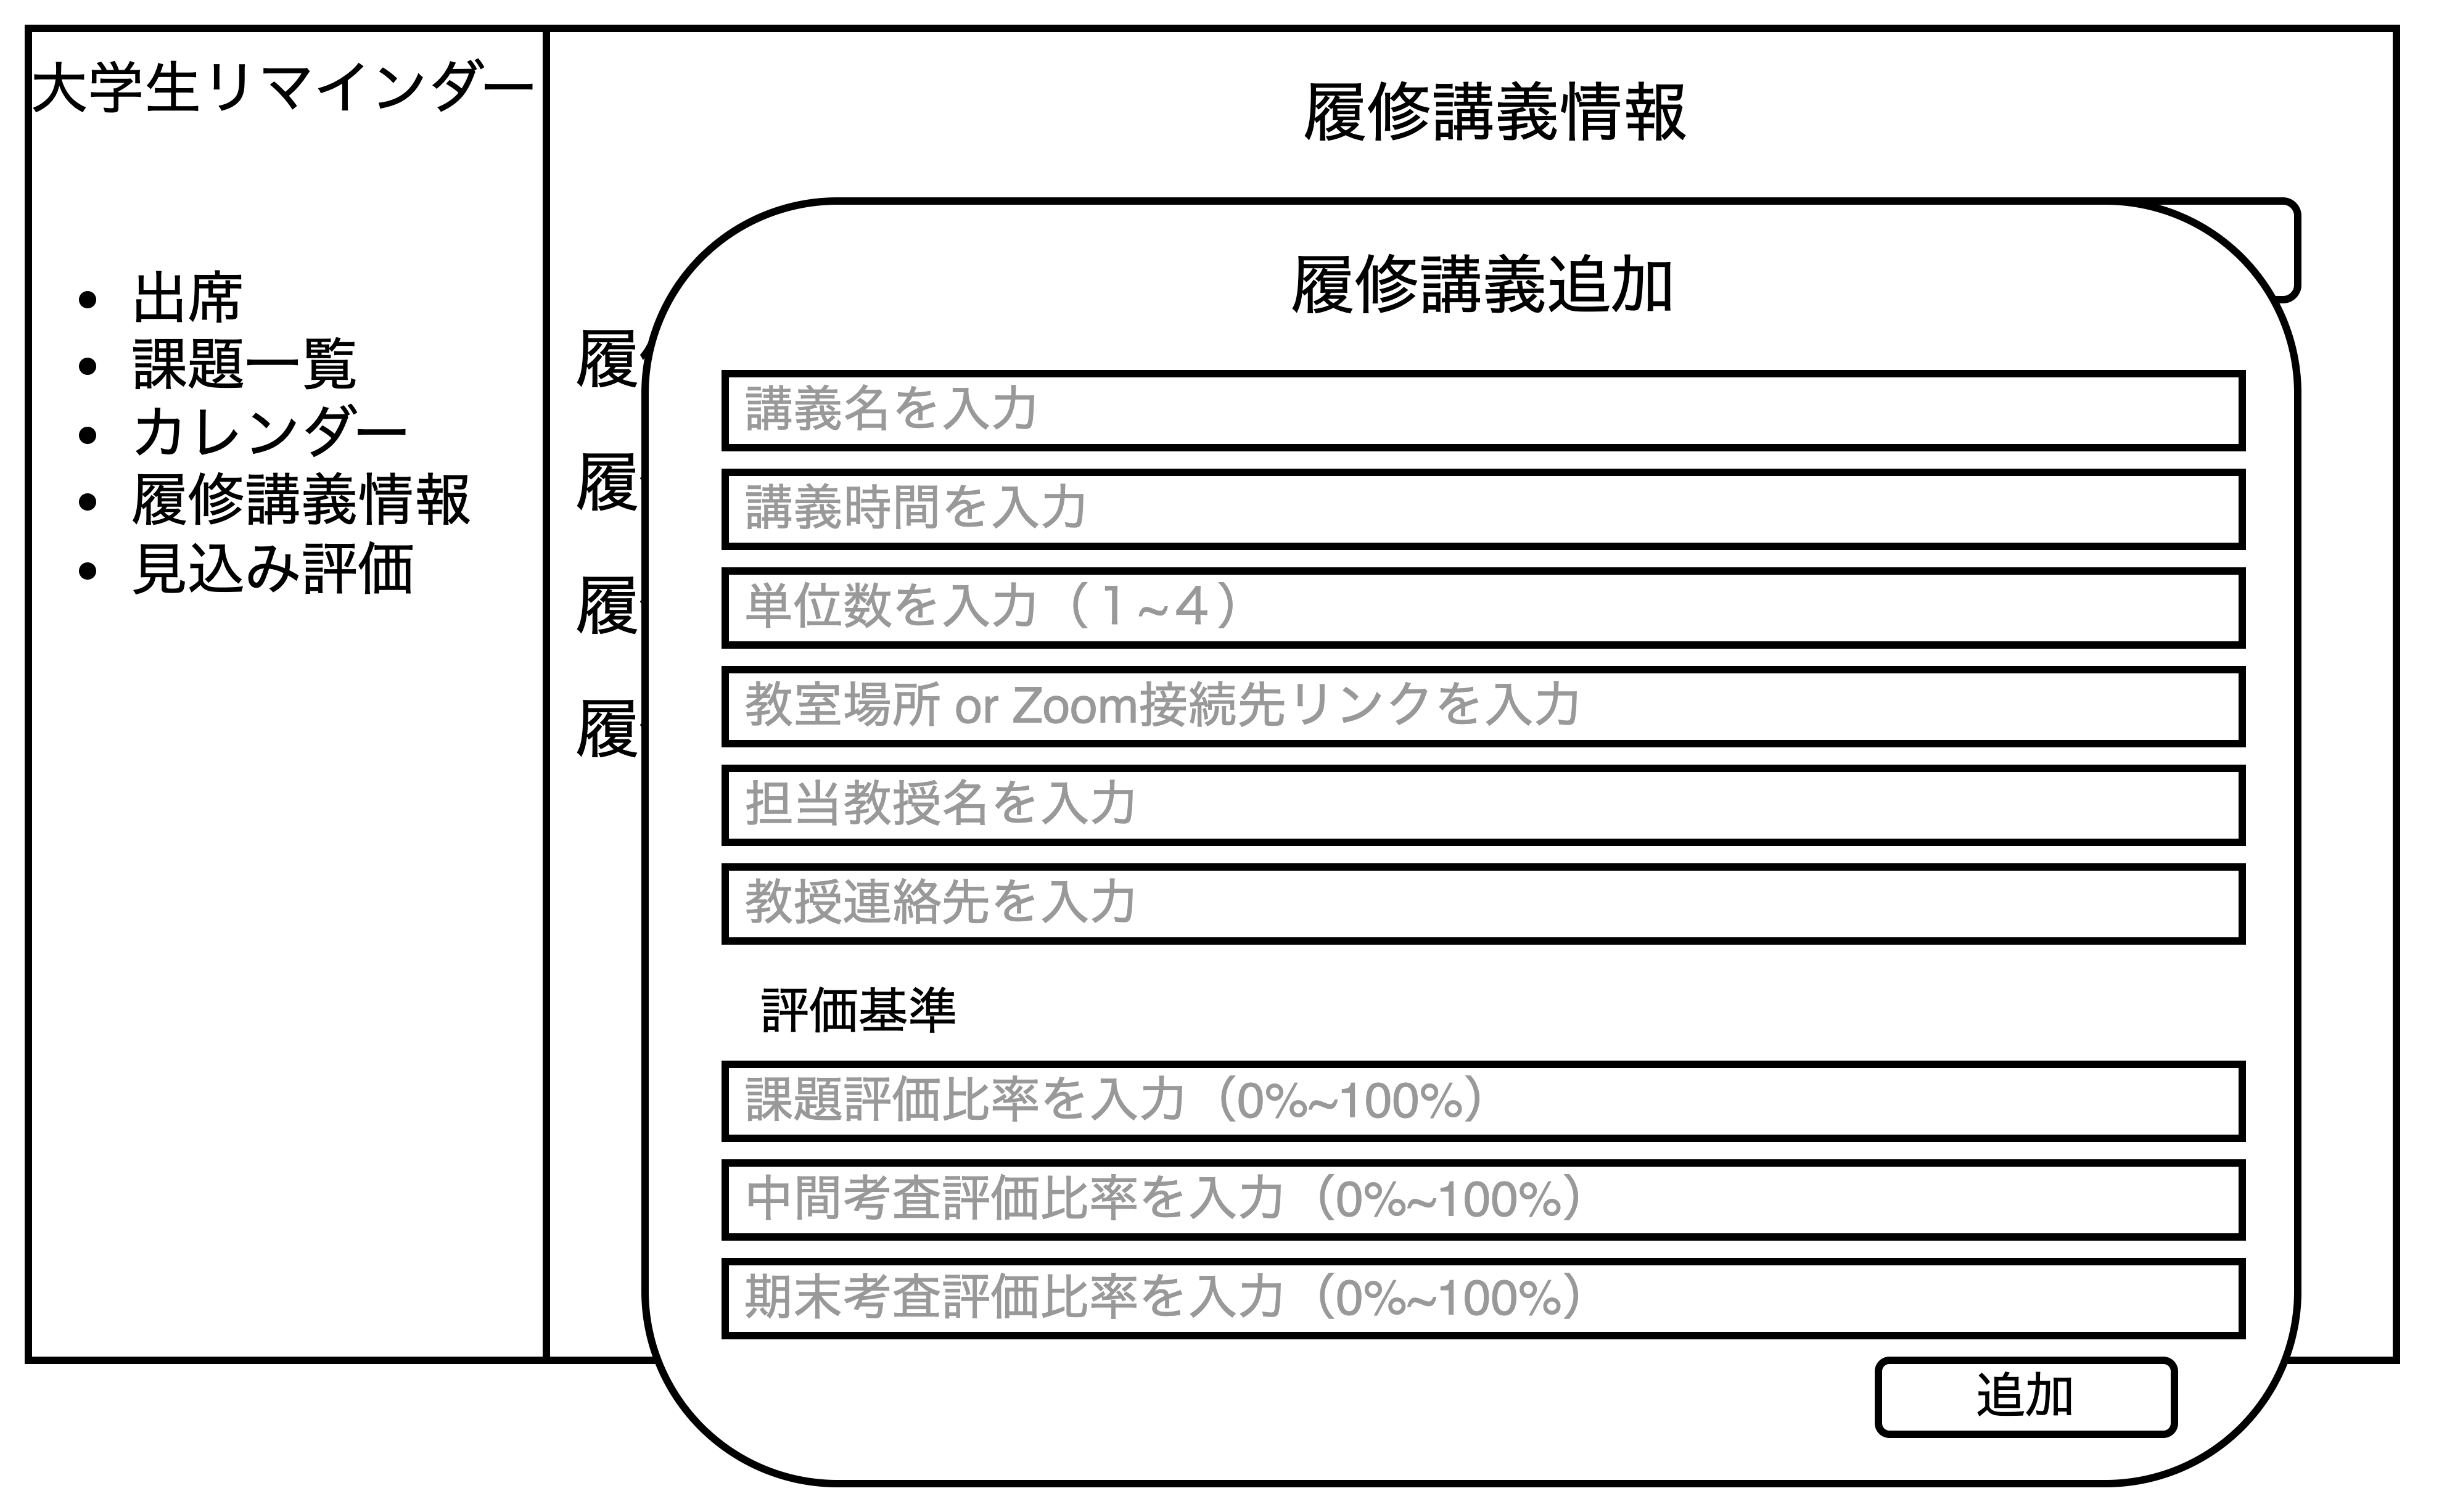
\includegraphics[width=120mm]{./img/Lecture2.png}
\caption{履修講義情報ページ(追加)}
\end{center}
\end{figure}
\begin{figure}[htbp]
\begin{center}
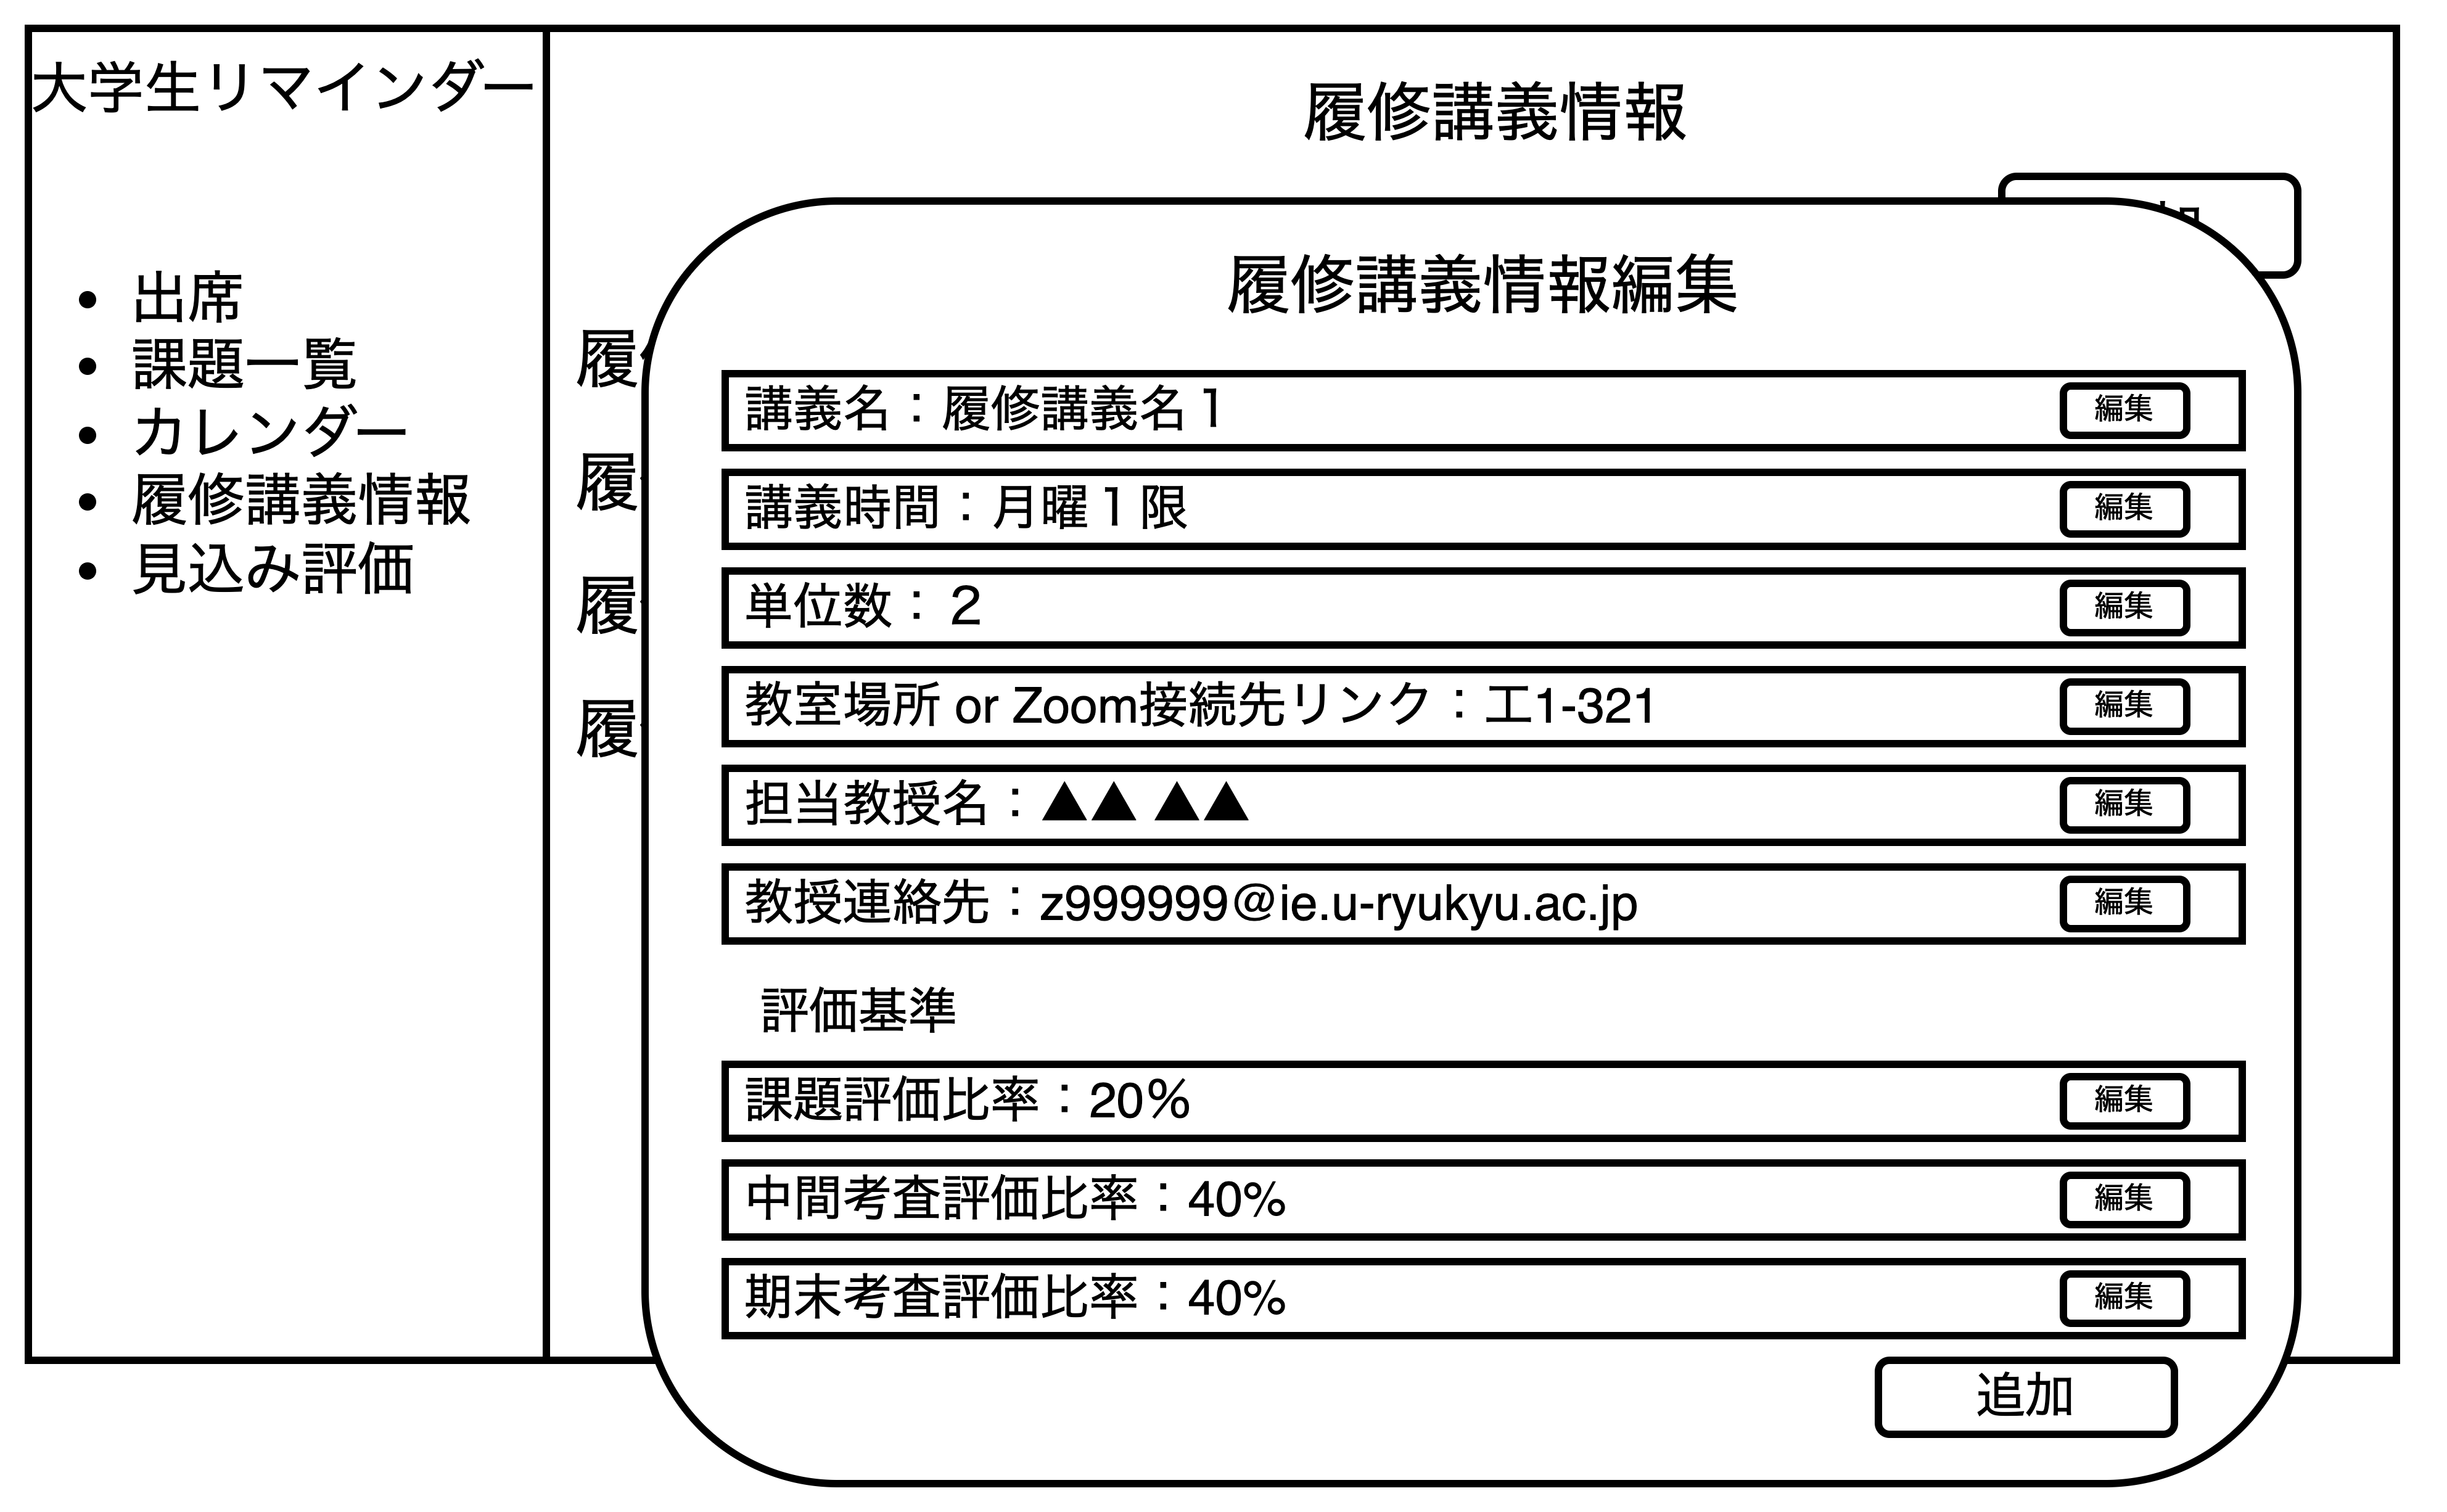
\includegraphics[width=120mm]{./img/Lecture3.png}
\caption{履修講義情報ページ(詳細・編集)}
\end{center}
\end{figure}

\clearpage

\subsubsection{見込み評価}
\begin{figure}[htbp]
\begin{center}
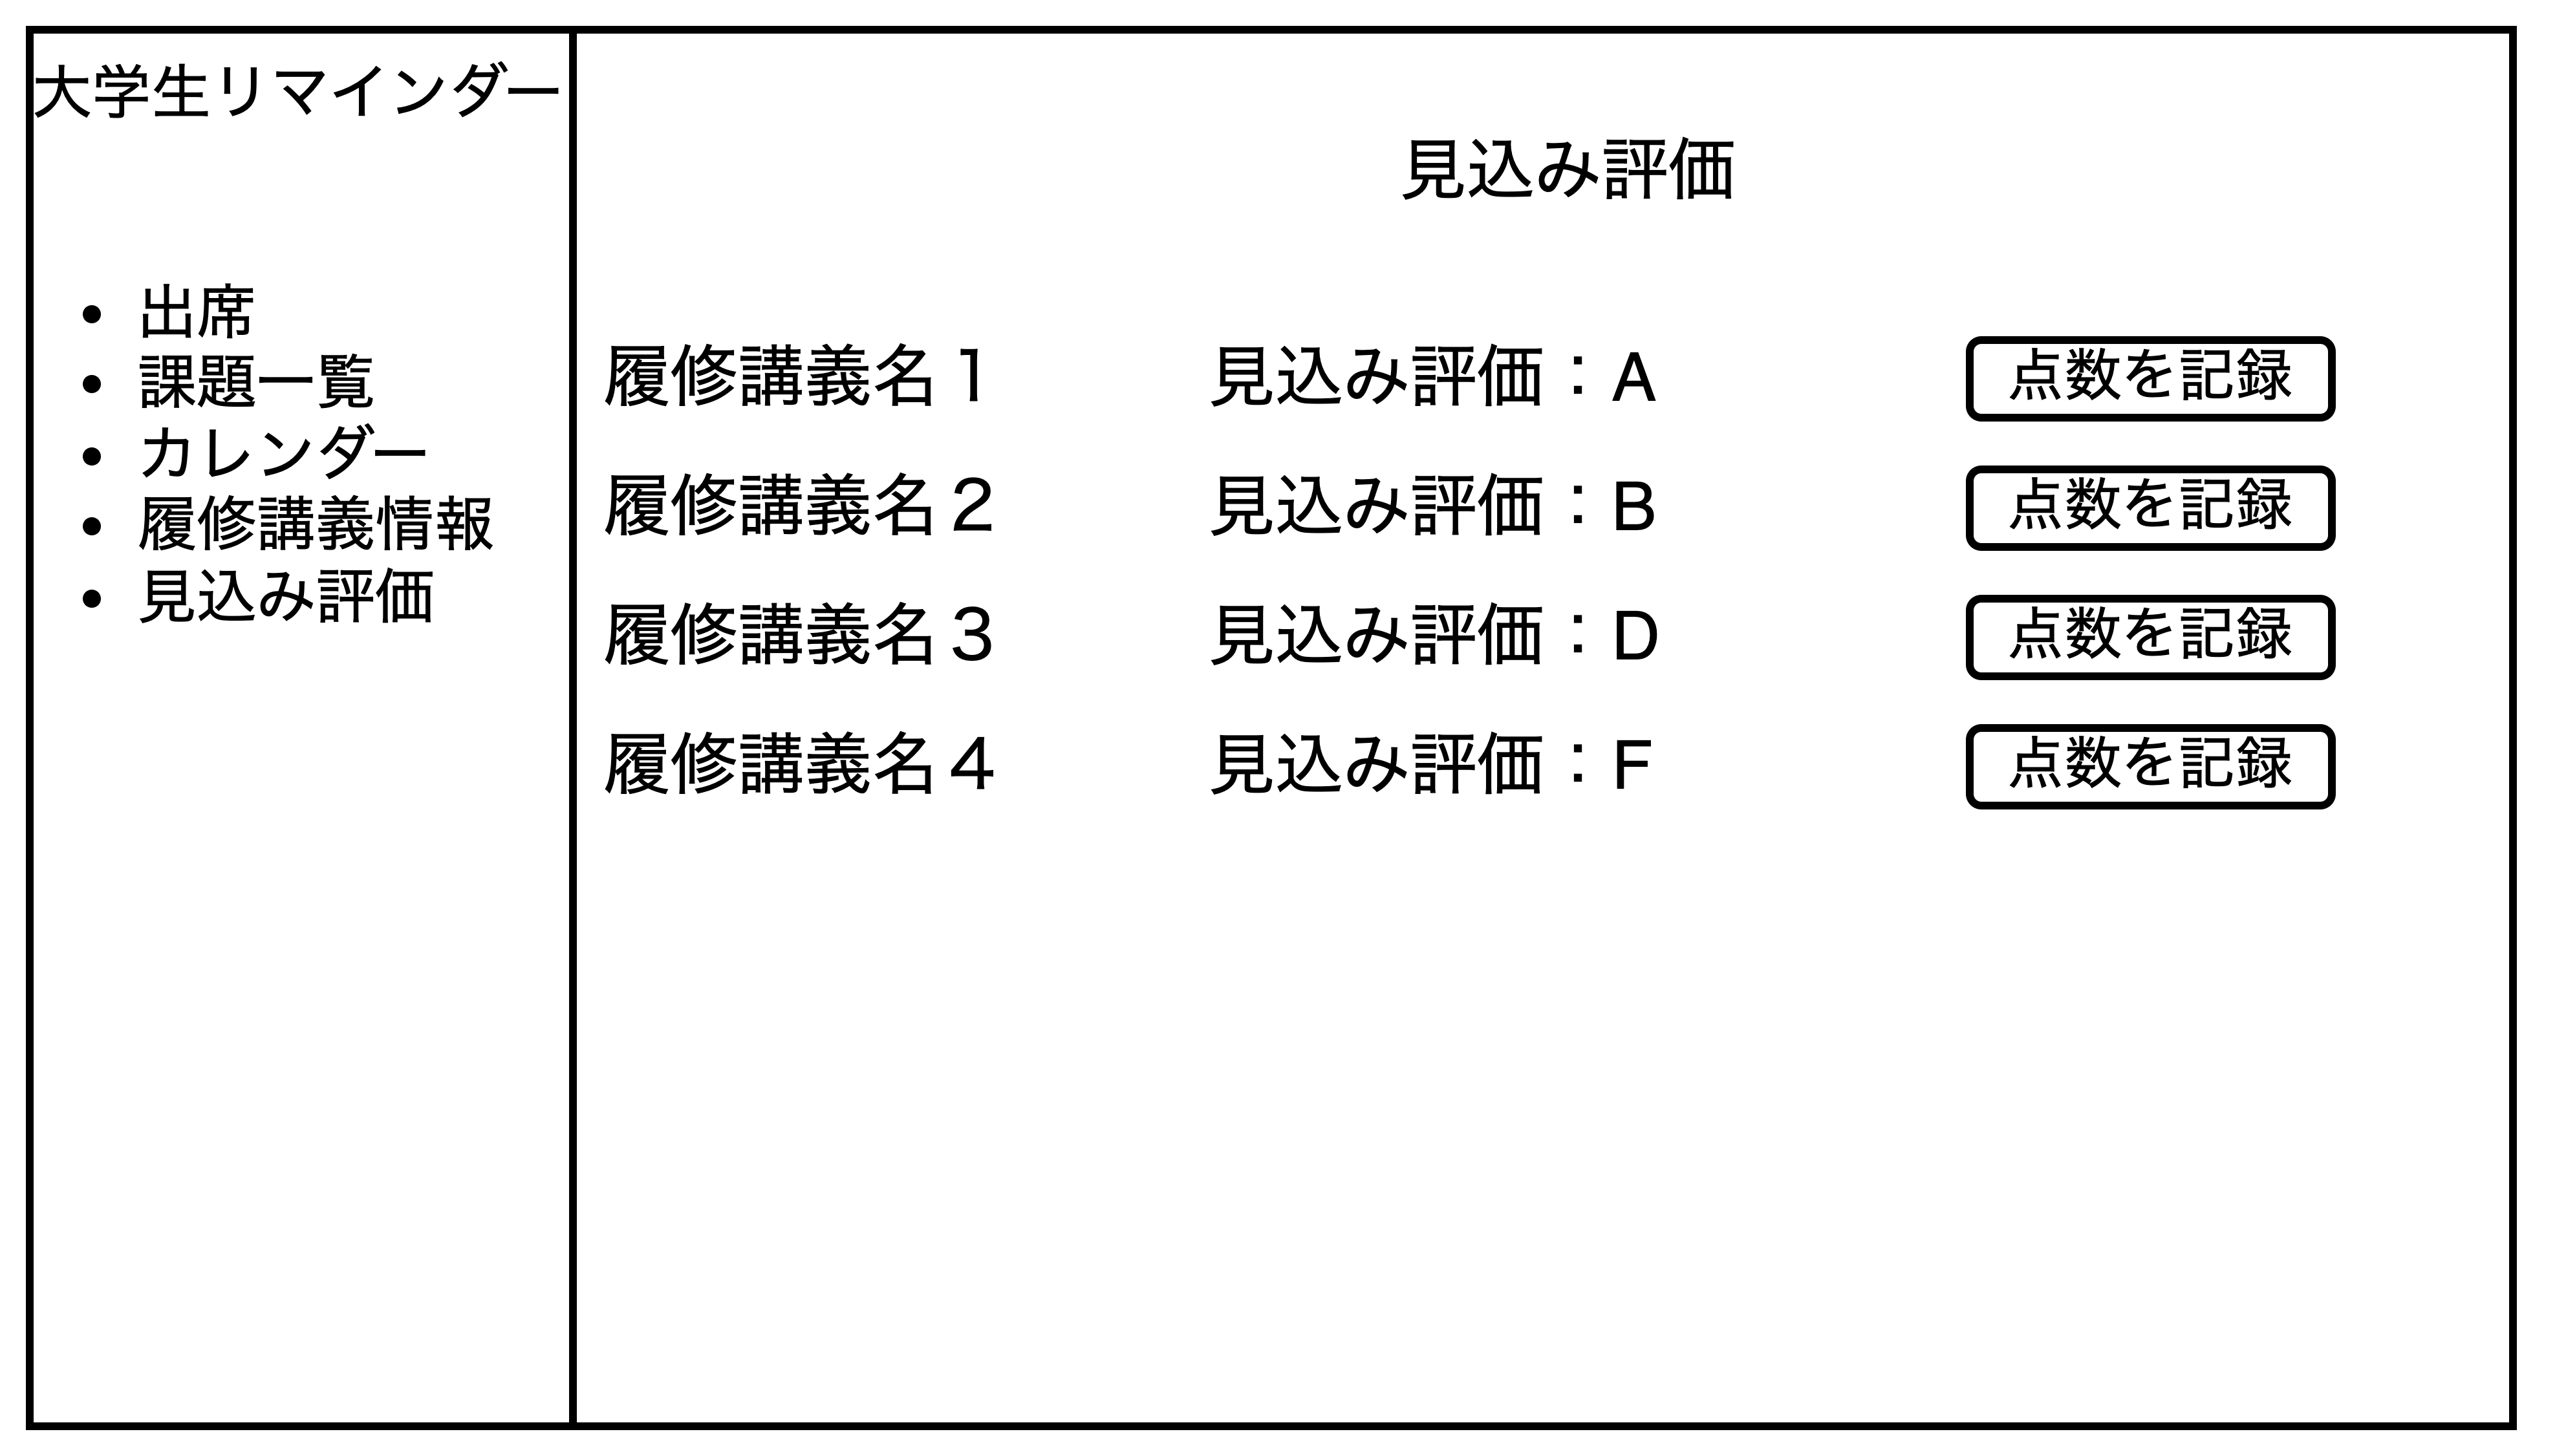
\includegraphics[width=120mm]{./img/Rating1.png}
\caption{見込み評価ページ(閲覧)}
\end{center}
\end{figure}
\begin{figure}[htbp]
\begin{center}
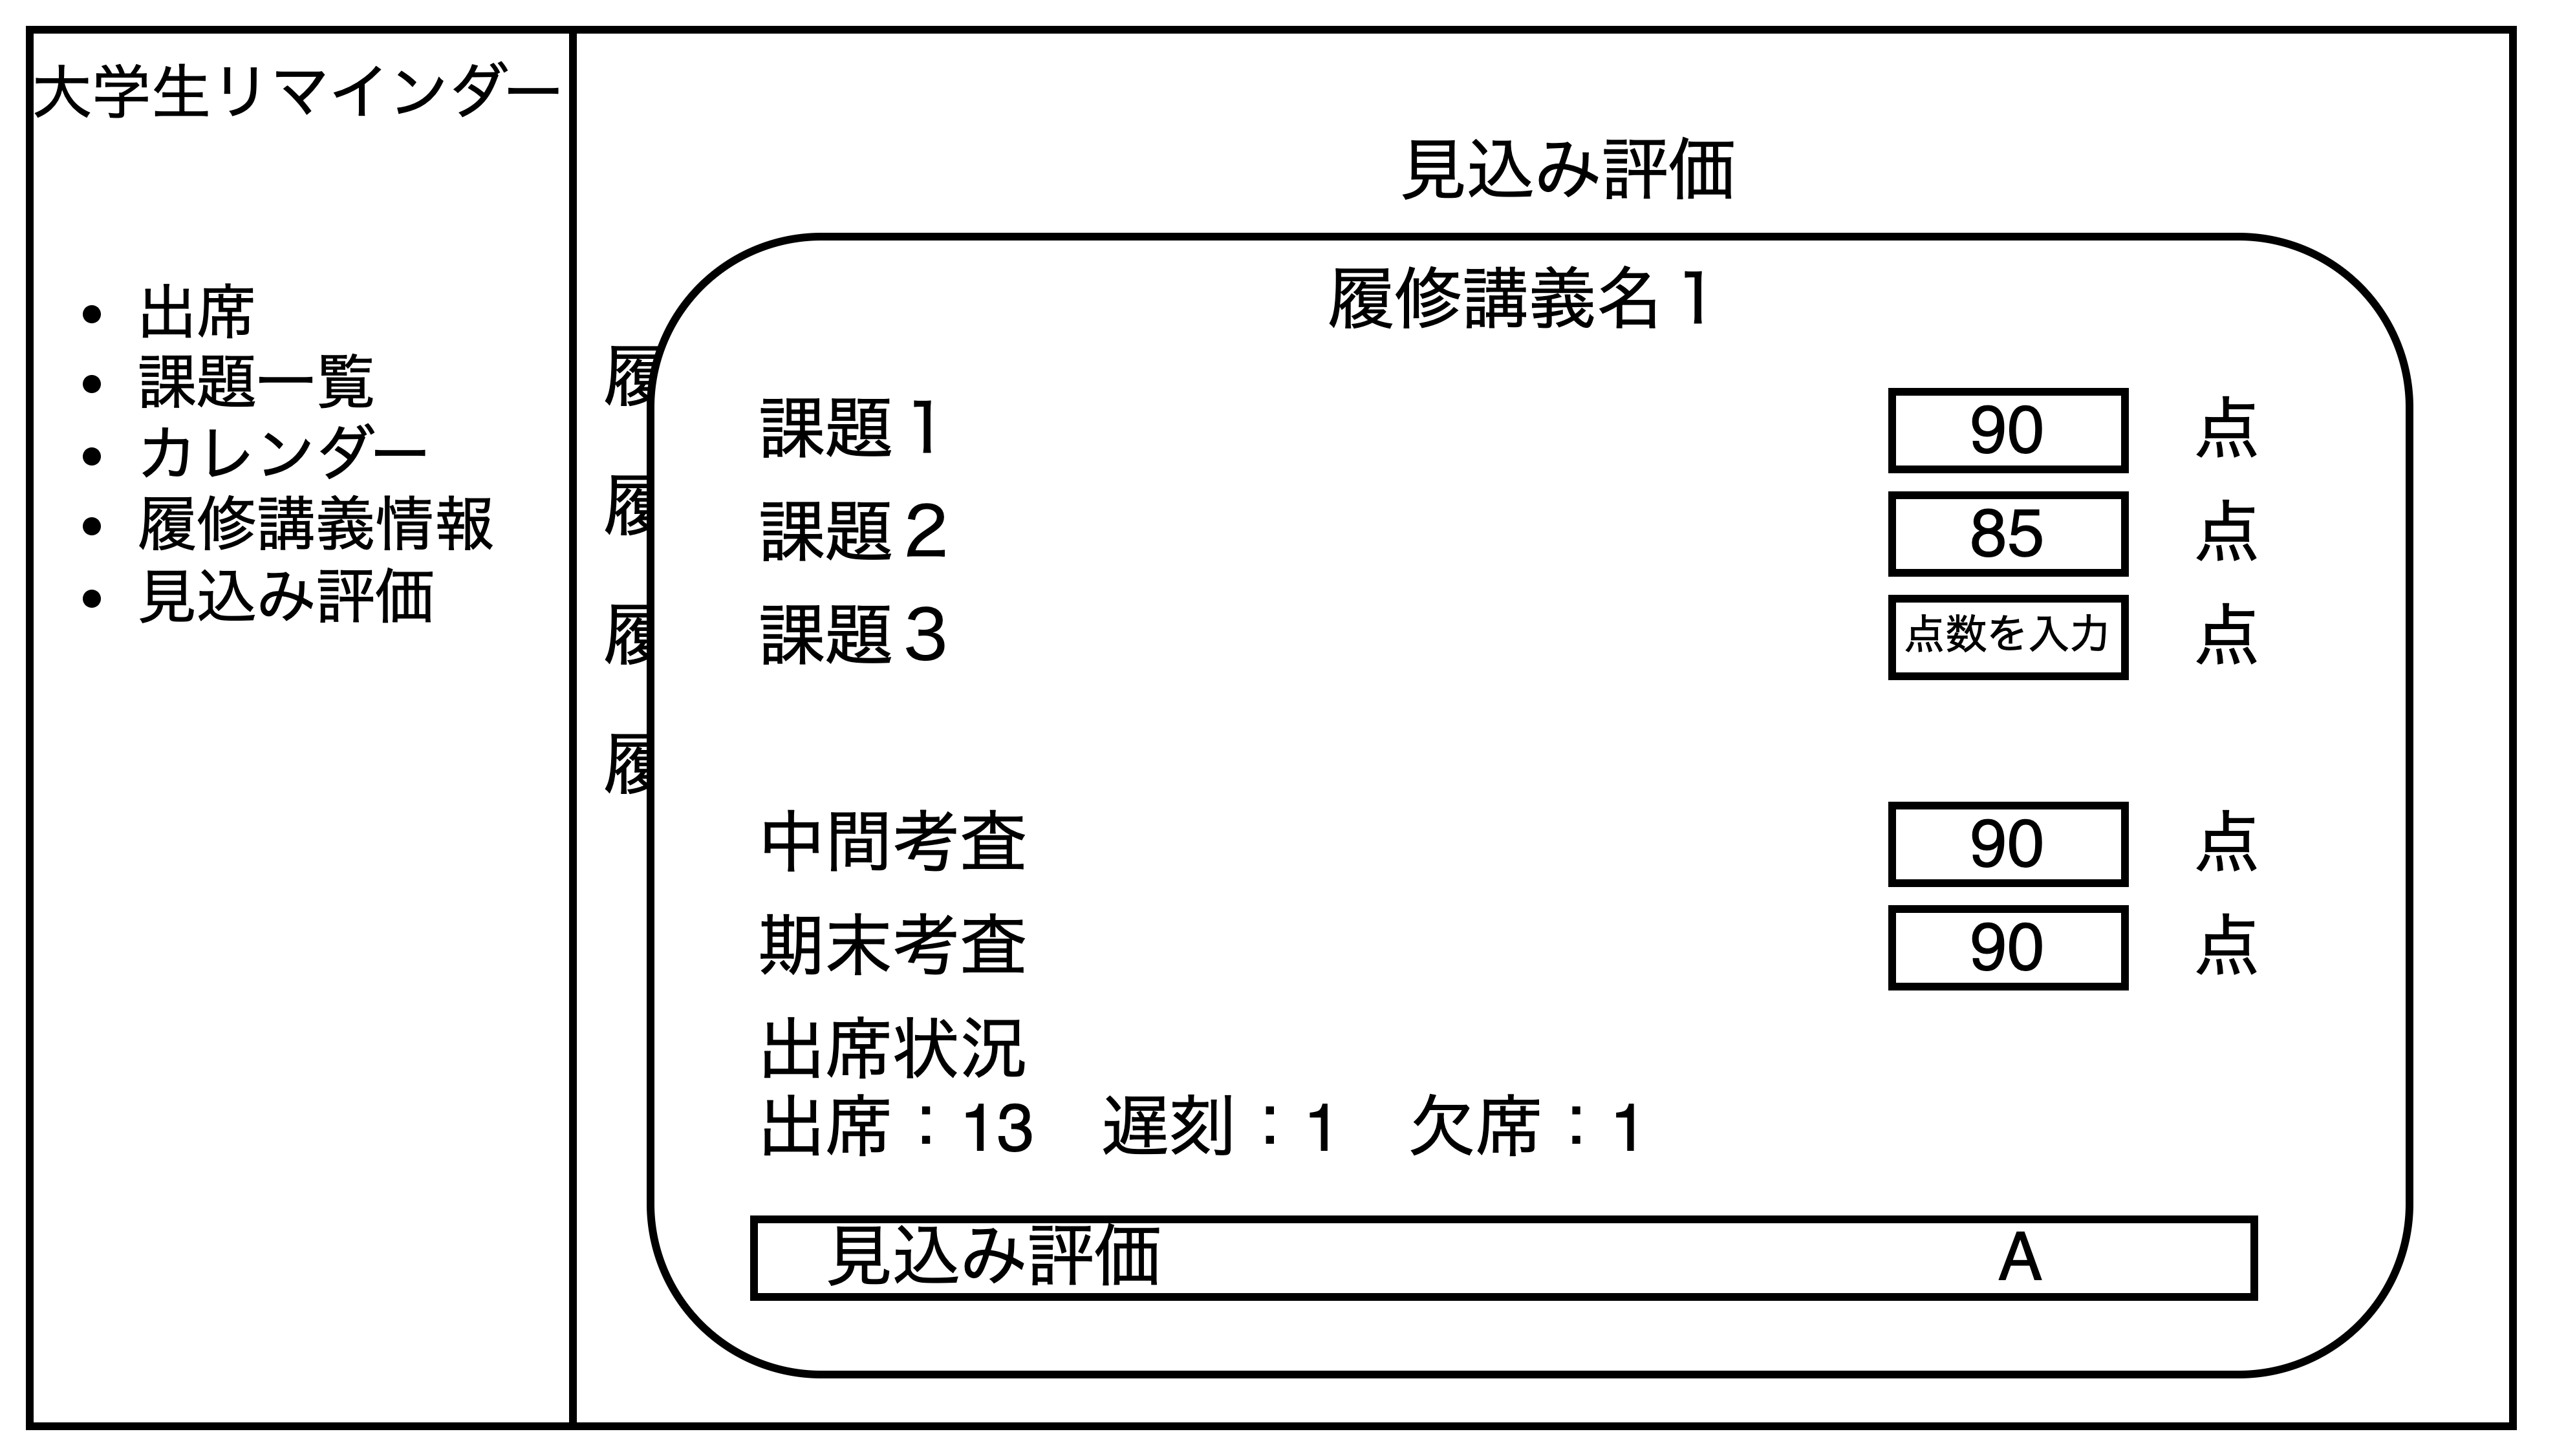
\includegraphics[width=120mm]{./img/Rating2.png}
\caption{見込み評価ページ(点数記録)}
\end{center}
\end{figure}

\subsection{データベース基本仕様}
\subsubsection{履修講義情報DB}
利用者が履修している講義情報を管理するデータベース。「講義名」「講義時間」「単位数」「教室場所 or Zoom接続先リンク」「教授情報」「評価基準」のデータを格納する。
\subsubsection{教授情報DB}
講義を担当する教授の情報を管理するデータベース。「教授名」「教授連絡先」のデータを格納する。
\subsubsection{出席情報DB}
講義の出席状況を管理するデータベース。「講義名」「講義日」「出席状況」のデータを格納する。
\subsubsection{課題情報DB}
講義ごとに出された課題の情報を管理するデータベース。「講義名」「課題名」「重要度」「締切日」「取組み予定日」のデータを格納する。
\subsubsection{課題評価情報DB}
課題・テストの点数の情報を管理するデータベース。「講義名」「課題名orテスト名」「点数」のデータを格納する。

\section{本課題の役割分担}
本課題の役割分担、作業時間は以下の通りである。
\begin{itemize}
\item 215710B 深村芽紅 - 仕様書作成 - 約5時間
\item 215724B 高里優菜 - 仕様書作成 - 約5時間
\item 215726J 神村琉恩 - 仕様書作成 - 約5時間
\item 215746C 新垣樹 - 仕様書作成 - 約5時間
\end{itemize}

\end{document}